\documentclass[]{kththesis}
\usepackage{csquotes} % Recommended by biblatex
\usepackage[style=numeric,sorting=none,backend=biber]{biblatex}
\usepackage[swedish]{babel}
\usepackage[]{graphicx}
\usepackage{float}


\graphicspath{{../images/}}

\addbibresource{references.bib}
\title{Image Classification of Real Estate Images with Transfer Learning}
\alttitle{Bildklassificering av fastighetsbilder med transfer learning}
\author{Oskar Råhlén och Sacharias Sjöqvist}
\email{orahlen@kth.se och sacsjo@kth.se}
\supervisor{Handledare}
\examiner{Examinator}
\programme{Degree project in Computer Science}
\school{School of Electrical Engineering and Computer Science}
\date{\today}

% Uncomment the next line to include cover generated at https://intra.kth.se/kth-cover?l=en
\kthcover{kth-cover.pdf}

% källor: \textcite och \parencite
\begin{document}
\frontmatter

\begin{abstract}
  Each minute, over 2 000 searches are made on Sweden’s largest real estate website. The site has over 20 000 apartments for sale in the Stockholm region alone. This makes the search-function a vital tool for the users to find their dream apartment, and thus the quality of the search-function is of significance. As of today, it’s only possible to filter and sort by meta-data such as numbers of room, living area, price, and location, but not on more complex attributes, such as “balcony” or “fireplace”. 
  
  To prevent the need for manual categorization of objects on the market, one option coud be to use images of the apartments as data-points in deep neural networks to automatically add rich attributes. This thesis aims to investigate if a high rate of success when classifying apartment images can be achieved using deep neural networks, specifically looking at the categories and attributes “balcony”, “fireplace”, as well as “type of room”. 
  
  Different types of architectures was compared amongst each other and feature extraction was compared against fine-tuning, in order to exhaustively investigate the thesis.
  
  The investigation showed that the “balcony-model” could determine if a balcony exists in an image, with a certainty of 98.1\%. For fireplaces, the maximum certainty reached was 85.5\%, which is significantly lower. The “type of room” classification reached a certainty of 97,9\%. 
  
  This all proves the possibility of using deep neural networks in order to classify and attribute real estate images.   
\end{abstract}

\begin{otherlanguage}{swedish}
  \begin{abstract}
    Varje minut görs 2000 sökningar på Sveriges största mäklarsite som har 20 000 bostadsrätter till salu bara i Stockholm.
    Detta ställer höga krav på sökfunktionen för att ge användarna en chans att hitta sin drömbostad. 
    Idag finns det möjlighet att filtrera på attribut såsom ”antal rum”, ”boarea”, ”pris” och ”område” men inte på attribut som ”balkong” och ”eldstad”.

    För att inte behöva kategorisera objekt manuellt för attribut såsom ”balkong” och ”eldstad” finns det möjlighet att använda sig av mäklarbilder samt djupa neurala nätverk för att klassificera objekten automatiskt.
    Denna uppsats syftar till att utreda om det med hög sannolikhet går att klassificera mäklarbilder efter ”balkong”, ”eldstad” samt ”typ av rum” med hjälp av djupa neurala nätverk.
    
    För att undersöka detta på ett utförligt sätt jämfördes olika arkitekturer med varandra samt feature extraction mot finetuning.
    Testerna visade att balkong-modellen med 98,1\% sannolikhet kan avgöra om det finns en balkong på någon av bilderna eller inte.
    För eldstäder nåddes ett maximum på 85,5\% vilket är väsentligt sämre än för balkonger.
    Under sista klassificeringen, den för rum, nåddes ett resultat på 97,9\%.

    Sammanfattningsvis påvisar detta att det är fullt möjligt att använda djupa neurala nätverk för att klassificera mäklarbilder. 
    

  \end{abstract}
\end{otherlanguage}
  
\tableofcontents

\mainmatter

\chapter{Introduktion}
Just nu finns över 20 000 bostadsrätter \parencite{hemnetstats} till salu på Sveriges största mäklarsite \parencite{hemnetom}, där nästan hälften av dessa ligger i Stockholm. Dit kommer 2,8 miljoner unika besökare varje vecka och gör tillsammans över 2000 sökningar i minuten \parencite{hemnetom}. Detta ställer höga krav på filtreringsfunktionerna för att potentiella köpare snabbt ska kunna hitta sin drömbostad. Idag erbjuds filtreringsfunktioner för bland annat antal rum, boarea, pris samt område. Det finns även möjligt att använda fritextsökning som hittar relevanta annonser beroende på texten som mäklaren skrivit i annonsen. En rekommendation av dessa sökord på bostadssidor är balkong, kakelugn och sjöutsikt.

Problemet med att bygga sökfunktionen på ord i texten till mäklarannonsen är att mäklaren måste nämna samtliga attribut som kan vara relevanta för eventuella köpare. Och det finns även en möjlighet för mäklaren att vara selektiv bland valda attribut. Det kan även uppstå problem med att synonymer används.

Genom att istället utgå från bilderna i annonsen kan det vara möjligt att hitta relevanta attribut, som till exempel balkong eller kakelugn, utan att det behöver nämnas i annonstexten. Det hade därför varit av stort intresse båda för bostadsplattformar och för människor som letar bostäder om det var möjligt att automatiskt koppla varje bild i en bostadsannons till ett antal attribut, vilket sedan kan underlätta bostadsletande. Det skulle även kunna utvecklas till attribut som idag inte är möjligt att söka efter, som takhöjd, skick och andra mer specifika egenskaper. Det skulle även finnas möjlighet att kombinera attribut, såsom skick och typ av rum, för att kunna göra ytterligare specifika sökningar.

Denna kategorisering av bilder från annonser skulle även kunna användas vid värdering av bostäder, vilket skulle i långa loppet leda till en jämnare prisnivå på bostäder och en tryggare affär för bostadsköpare. Detta då det skulle vara enklare att jämföra priser mellan bostäder om det finns fler attribut att jämföra.

För att på ett automatiskt tillvägagångssätt koppla attribut till bilder i bostadsannonser behövs någon form av bildkategorisering. Vi har därför valt att studera vilka metoder inom maskinlärning och i huvudsak djupinlärning som kan användas för att kategorisera dessa typer av bilder. Dessa modeller behöver vanligtvis tränas med en stor mängd data och det behövs experiment för att avgöra dess tillförlitlighet. För att sedan kunna använda bilder från bostadsannonser som indata för att generera alla önskade attribut.

\section{Syfte}
Syftet med studien är att undersöka vilka tekniker inom maskininlärning som kan användas för att hitta relevanta attribut i bilder från bostadsannonser vilket sedan kan användas som nyckelord vid sökningar av bostadsannonser.

\section{Frågeställning}
Går det med tekniker inom maskininlärning att hitta relevanta attribut i bilder från bostadsannonser?

\section{Avgränsningar}
Studien kommer undersöka möjligheten att hitta tre olika attribut: balkong, eldstad samt typ av rum. Typ av rum är begränsat till kök, badrum och sovrum. Vi har även valt att avgränsa oss till annonser för bostadsrätter i Stockholm samt på tekniker inom maskininlärning. 

Dessa avgränsningar görs framförallt för att marknaden efterfrågar denna typ av modell samt att det inte fanns oändligt med resurser. Att generera träningsdata för dessa attribut kommer vara krävande nog, därför togs inte flera attribut med.

Anledningen till att avgränsa sig till bostadsrätter i Stockholm är att vi vill ha lägenheter som är i ungefär samma miljö och typ av människor som bor där, för att inte behöva ha allt för mycket träningsdata. 



\chapter{Bakgrund}

\section{Bildklassificering}
Klassificering av objekt i bilder är område där forskningen har gjort stora framsteg senaste åren \parencite{Goodfellow-et-al-2016}. Att applicera teknikerna inom klassificering av bilder från mäklare har skett i ett fåtal tidigare studier \parencite{cao2019classification} \parencite{poursaeed2018vision}. Dessa studierna har dock utgått ifrån hus i andra länder än Sverige och istället fokuserat på att utifrån bilderna estimera slutpris på fastigheterna. Detta skiljer sig från vårt arbete, där det huvudsakliga syftet är att hitta attribut i bilderna, vilket i ett senare skede kan användas i en prisestimering. Det har även studerats möjligheten till att klassificera scener med hjälp av bilder. \cite{zhou2014learning} har byggt modeller som klassificerar 67 olika typer av svener inomhus. 

\section{Maskininlärning}
Maskininlärning är ett sätt att programmera datorer så de optimerar ett problem med hjälp av exempeldata eller tidigare erfarenhet \parencite{alpaydin2009introduction}. Maskininlärning är ett aktivt forskningsfält inom datalogi. Lärandeprocessen för en maskininlärningsalgoritm kan se ut på följande sätt: Ett datorprogram har som uppgift att lära sig en förutbestämd uppgift T, hur väl den gör detta, algoritmens prestanda, är måttet P. Till sin hjälp har datorprogrammet tidigare erfarenhet E. Om prestandan P blir högre då vi tillför erfarenheten E till programmet, då lär sig programmet.

Maskininlärningsmodeller kan delas in i två kategorier, övervakat lärande (eng. supervised learning) och oövervakat lärande (eng. unsupervised learning) \parencite{murphy2012machine}. Vid övervakat lärande är erfarenheten E redan kategoriserad och uppmärkt för uppgiften T, vid oövervakat lärande så är den inte det. Ett exempel är en maskininlärningsmodell som har som uppgift T att kategorisera bilder i vissa förutbestämda kategorier. Vid övervakat lärande kommer erfarenhet E bestå av bilder som redan är uppmärkta med rätt kategori. Modellen ska då med hjälp av erfarenheten kunna kategorisera nya data som inte är uppmärkt. 

\section{Artificiella  neurala nätverk}
En samling algoritmer inom maskininlärning med många tillämpningsområden är artificiella neurala nätverk (ANN). Enligt \textcite{Goodfellow-et-al-2016} så var ANN från början ett försök till att bygga en digital modell av det biologiska neuronsystemet. Forskningen inom områden avvek dock snabbt från att efterlikna den biologiska varianten och fokuserade istället på att öka prestandan på maskininlärningsproblem. De minsta byggstenarna i ANN, neuronen, fungerar fortfarande som dess biologiska variant. Ett neuron får signaler in och skickar sedan signaler ut via synapserna. Hur stark utsignalen bör vara simuleras i en dator med hjälp av vikter (eng. weights), även kallat för parametrar. Varje neuron i nätverket har sina tillhörande vikter. När ett ANN tränas så görs detta genom att justera dessa vikter \parencite{Goodfellow-et-al-2016}. De viktade insignalerna bör även nå upp till en viss tröskel för att en utsignal ska skickas, detta simuleras i ANN med aktiveringsfunktioner. ANN är en acyklisk graf som består av dessa artificiella neuroner.

\begin{figure}[h]
  \centering
  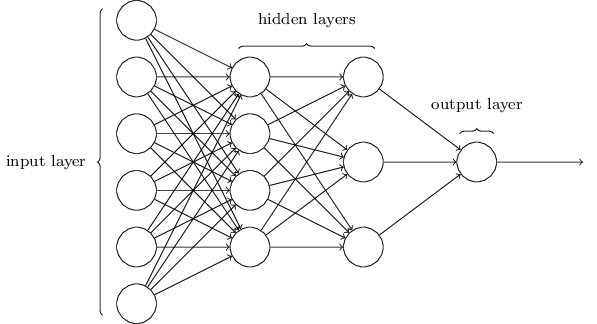
\includegraphics[width=0.6\textwidth]{nn}
  \caption{En illustration över ett artificiellt neuralt nätverk \parencite{nielsen2015neural}.}
\end{figure}

Ett ANN består först av ett indatalager (eng. input layer). Indatalagret representeras av ett neuron per kännetecken (eng. features) i indata. Då indata är bilder motsvarar ett neuron i indatalagret en pixel i bilden. Indatalagret är sedan ihopkopplat med ett nytt lager med neuroner. Det kan vara flera lager efter varandra och dessa kallas för de gömda lagren (eng. hidden layers). De gömda lagren kan bestå av godtyckligt många neuroner och de behöver inte ha samma antal neuroner. Efter de gömda lagren kommer utdatalagret (eng. output layer). Antalet neuroner i utdatalagret bör motsvara formen på den utdata vi vill ha. Om modellen ska kategorisera bilder i tio olika kategorier, bör utdatalagret innehålla tio neuroner. Det är värdet dessa neuroner i utdatalagret har som är svaret från vårt ANN.

Ett ANN blir bättre på att utföra sin uppgift genom att ändra sina vikter. Detta sker i två steg, feed-forward pass och backward pass, även kallat för backpropagation \parencite{alpaydin2009introduction}. Vid feed-forward skickas träningsdata (som kommer från tidigare erfarenhet E) in i nätverket för att få ut ett svar. Då all träningsdata är uppmärkt så jämförs svaret från nätverket med det korrekta svaret. Utifrån antal fel och hur fel nätverket hade, beräknas en kostnad. Denna kostnad kan beräknas på olika sätt men vanligtvis används funktionen cross-entropy loss \parencite{Goodfellow-et-al-2016}. Målet är att träna modellen så denna kostnad blir så låg som möjligt. Nästa steg är backward pass. Vi vill ändra vikterna så att kostnaden blir lägre, detta görs genom att beräkna gradienten av kostnaden med avseende på alla vikter. Vi tar sedan ett steg åt motsatt håll till gradienten för att minska kostnaden. Storleken på detta steg kallas för inlärningstakt (eng. learning rate).

Vanligtvis delas all träningsdata in i högar, vilket kallas för mini-batch \parencite{Goodfellow-et-al-2016}. Istället för att beräkna gradienten för varje datapunkt så beräknas gradienten för en hel mini-batch för att sedan använda sig av en genomsnittlig gradient. En epok (eng. epoch) är när nätverket har gått igenom alla datapunkter i träningsdatamängden. Hur många träningssteg detta innefattar beror på antal datapunkter samt storleken på mini-batch.

\subsubsection{Stochastic gradient descent}
Det finns olika algoritmer för exakt hur vikterna ska ändras när ett ANN tränas. En av de vanligaste algoritmerna är Stochastic Gradient Descent (SGD) \parencite{Goodfellow-et-al-2016}. Den bygger på feed-forward pass och backward pass men beräknar gradienten på ett fåtal slumpmässigt utvalda datapunkter istället för alla datapunkter i den befintliga träningsdata \parencite{bottou2010large}. Anledningen är att effektivisera modellen så träningen går snabbare. En variant är mini-batch SGD, där samma principer appliceras på en mini-batch istället för all träningsdata.

En vidareutveckling är SGD med momentum \parencite{qian1999momentum}. Algoritmen med momentum kommer ihåg förändringen av vikterna vid föregående iteration och baserar nästa uppdatering på en linjärkombination av gradienten och den tidigare förändringen. Denna teknik har fått stor genomslagskraft inom forskningen av ANN \parencite{sutskever2013importance}.

\section{Neurala nätverk med konvolution}
Neurala nätverk med konvolution (eng. Convolutional Neural Network, CNN) är en viss typ av neurala nätverk som fungerar bra då indata kan ses som ett rutnät \parencite{Goodfellow-et-al-2016}. Detta inkluderar data om tidsserier, som kan ses som ett endimensionellt rutnät, men också bilder, som kan ses som ett rutnät av pixlar. CNN introducerades för 20 år sedan men det har, på grund av begränsningar i hårdvara och arkitekturer, inte gått att träna djupa CNN förrän för några år sedan \parencite{huang2017densely}. Enligt \textcite{huang2017densely} har CNN idag blivit den dominanta tekniken inom maskininlärning för igenkänning av visuella objekt. Och enligt \textcite{simon2016imagenet} är CNN som är förtränade på bilder från ImageNet grunden till majoriteten av state-of-the-art-modeller inom bildkategorisering.

\subsection{Lager}
Det finns några grundläggande lager som används i de flesta typer av CNN, oberoende av arkitektur. CNN kan användas för många olika typer av indata men vi har här valt att fokusera på dess tillämpningar med bilder. En vanlig uppbyggnad av ett CNN för bildkategorisering är indatalager, konvolutionslager, ReLU, föreningslager och sist ett FC-lager.

\subsubsection{Indatalager}
Detta lager innehåller pixelvärden från bilden som skickas in i nätverket. Vanligtvis används RGB-bilder, vilket betyder att varje pixel även har tre färgkanaler. Storleken på bilden beror på arkitektur men vanligast är formatet som används i ResNet-arkitekturen, vilket är 224 pixlar i höjd och 224 pixlar i bredd \parencite{krizhevsky2012imagenet}. Storleken på tensorn som innehåller indata motsvarande en bild har då storleken 224 x 224 x 3. Alla arkitekturer som fått större spridning tar alltid en kvadratisk bild som indata.

\subsubsection{Konvolutionslager}
En konvolutionslager består av en godtycklig mängd filter med träningsbara vikter \parencite{lecun1995convolutional}. Varje filter är kvadratiskt och brukar vara små i höjd och bredd med samma djup som indata till lagret. Ett exempel på filterstorlek är 5 x 5 x 3 \parencite{krizhevsky2012imagenet}. Vid feed-forward pass så glider vi detta filter över bilden som är vårt indata. Vi beräknar skalärprodukten av filtret och den mängd pixlar av bilden som filtret ligger över. Efter beräkningen glider vi filtret åt sidan \parencite{he2015spatial}. Vanligtvis skjuts filtret en pixel i taget, men det kan skilja mellan lager. Utdata från varje filter blir en tvådimensionell aktiveringskarta (eng. activation map). Höjd och bredd på utdata från ett konvolutionslager beror på tre hyperparametrar: Antal filter, kliv (eng. stride) och nollutfyllnad (eng. zero padding). Antal filter motsvarar djupet på utdata. Kliv bestämmer antal pixlar vi förflyttar oss vid varje glidning och nollutfyllnad avgör om vi skapar en ram runt indata med nollor och i sådana fall hur tjock den ramen är. Klivstorlek och nollutfyllnad avgör dimensionerna på utdata.

\subsubsection{Aktiveringslagret ReLU}
Aktiveringslagret (eng. activation layer) består av en aktiveringsfunktion. Denna funktion ska motsvara den tröskel som finns i biologiska neuroner för att trigga en utsignal. En av de vanligaste aktiveringsfunktionerna inom djupinlärning för bildkategorisering är Rectified Linear Units (ReLU) \parencite{krizhevsky2012imagenet}. Aktiveringsfunktionen appliceras elementvis och ReLU applicerar funktionen \begin{equation} f(x) = max(0,x) \end{equation} på varje element i indata till lagret. Det betyder att varje element som är positivt är opåverkat och varje negativt värde får värdet noll. Storleken på datamängden blir oförändrad.

\subsubsection{Föreningslager}
Ett föreningslager (eng. pooling layer) applicerar en nedsampling (eng. downsampling) på indata \parencite{krizhevsky2012imagenet}. Detta sker längs de spatiala dimensionerna bredd och höjd. Vanligtvis sker detta för att minska antalet parametrar i nätverket och för att minska beräkningskraften som behövs för att träna nätverket. Det är även en teknik för att undvika överanpassning (eng. overfitting). Det som främst används inom CNN är max pooling. Det är när ett förutbestämt område, till exempel 2 x 2 pixlar, sammanfattas genom att det högsta värdet av dessa fyra pixlar väljs ut. Max pooling med filter i storlek 2 x 2 och klivstorlek 2 är vanligt förekommande. Indata minskar då i storlek med 75\%.

\subsubsection{FC-lager}
Det lager som är vanligt förekommande i traditionella neurala nätverk är FC-lagret (eng. Fully-connected layer) \parencite{krizhevsky2012imagenet}. I detta lager har varje neuron en koppling till alla aktiveringar från det tidigare lagret. Dessa neuroner har tillhörande träningsbara vikter, som vanligtvis sparas i en matris \parencite{Goodfellow-et-al-2016}. Detta möjliggör även effektiva implementationer med matrismultiplikation. Storleken på utdata beror på storleken på viktmatrisen. I CNN är det vanligt förekommande att det sista lagret är ett FC-lager som byggs på det sättet att formen på utdata motsvarar antal kategorier modellen ska kunna kategorisera i. Ett exempel är att om en bild ska klassificeras bland tio klasser, så kan utdata från sista lagret ha formen 10 x 1.

FC-lager som används i slutet av nätverk brukar även kombineras med ett softmax-lager. Ett softmax-lager gör att de olika utdatavärdena kan ses som en distribution \parencite{Goodfellow-et-al-2016}.

\subsection{Tekniker inom djupinlärning}
Det har uppkommit vissa tekniker inom djupinlärning som inte är en del av arkitekturer inom CNN men som ofta används med moderna modeller för att uppnå höga resultat. Två populära tekniker är batch-normalisering och dataförstärkning.

\subsubsection{Batch-normalisering}
Att träna djupa neurala nätverk är komplicerat då distributionen av varje lagers indatavärden förändras under träning \parencite{ioffe2015batch}. Detta leder till att träningen av nätverket tar längre tid, då vi behöver använda långsammare inlärningstakt. Det leder också till att viktinitieringen blir väldigt finkänslig. Enligt \textcite{ioffe2015batch} kallas detta fenomen för internal covariate shift och löses genom att normalisera indata till varje lager. Metoden bygger på att normaliseringen blir en del av arkitekturen och där en normalisering sker för varje mini-batch av vårt träningsdata. Denna typ av batch-normalisering tillåter oss att använda högre inlärningstakt och gör att initieringen av vikterna inte blir lika kritisk. Det fungerar även som regularisering (eng. regularization), vilket gör att andra tekniker för regularisering kan uteslutas.

Batch-normalisering har visat sig vara extra viktigt för lyckad träning och för att större nätverk ska konvergera, nätverk som VGG19 \parencite{simon2016imagenet}. Det har även visat sig att den högre inlärningstakten, som batch-normalisering tillåter, leder till en högre slutlig noggrannhet än vad som annars hade varit möjligt \parencite{simon2016imagenet}. Tidigare experiment har visat att detta har fungerat både bland annat AlexNey och VGG19 \parencite{simon2016imagenet}.

\subsubsection{Dataförstärkning}
Djupa neurala nätverk behöver en stor mängd data för att lära sig effektivt. Insamlingen av denna data är oftast dyrt och tidskrävande. Dataförstärkning (eng. data augmentation) löser detta genom att öka datamängden artificiellt genom att göra förändringar på befintlig data \parencite{taylor2017improving}. Det har visat sig att generell dataförstärkning leder till ökad prestanda på de flesta CNN. En viktig del av dataförstärkningen är att indata fortfarande ska tillhöra samma klass som den tillhörde innan. Inom bildkategorisering sker förändringen med geometriska och fotometriska transformationer. Geometriska transformationer ändrar geometrin i bilden med målet att vårt CNN ska vara oberoende av objektets position eller orientering. Dessa transformationer inkluderar att flippa, beskära, skala och rotera bilden. Fotometriska transformationer förändrar istället färgkanalerna och målet är att vårt CNN ska vara oförändligt till skillnader i belysning och färg. 

\subsection{Arkitekturer}
Här presenteras ett urval av de mest betydelsefulla arkitekturerna inom CNN för bildkategorisering. En tydlig trend är att CNN har fått fler lager, blivit djupare, med tiden. Från LeNet \parencite{lecun1998gradient} med fem lager, till VGG med 19 lager \parencite{simonyan2014very} och Residual Networks (ResNet) med över 100 lager \parencite{he2016deep}. Ett problem med detta är att viktig information i indata försvinner innan det hinner nå slutet av nätverket \parencite{huang2017densely}. Det har därför kommit arkitekturer som försöker lösa detta problem. ResNet löser det genom att förbikoppla vissa lager med identitetskopplingar. DenseNet skapar istället flera olika förbikopplingar inne i nätverket.

\subsubsection{ResNet}
ResNet är en arkitektur för CNN som består av konvolutionslager, föreningslager och FC-lager \parencite{he2016deep}. ResNet finns i olika varianter, från ResNet18 till ResNet152, och skillnaden är storleken på nätverket, där ResNet18 består av 18 lager. Efter utvecklingen av djupare CNN så nådde till slut ett tak för hur kraftfulla modellerna kunde vara. ResNet är en lösning på det här problemet som introducerar identity shortcut connections. Det betyder att det finns kopplingar som hoppar över vissa konvolutionslager, vilket betyder att om nätverket tycker att vissa lager är onödiga så kan den helt enkelt skippa dessa. Anledningen till namnet är att dessa kopplingar skickar vidare identiteten av indata till nästkommande lager. Dessa kopplingar leder till att nätverken kan göras oändligt stora utan prestandaförlust, för modellen kan alltid använda identiteten. Modeller med dessa residuala funktioner ska även vara enklare att optimera \parencite{he2016deep}. ResNet-modellen tar RGB-bilder i storleken 224 x 244 pixlar som indata och målet är att kategorisera bilden bland 1000 kategorier från ImageNet. ResNet18 består först av ett konvolutionslager och sedan ett max pooling-lager. Därefter kommer en stack med konvolutionslager där det även sker en nedsampling med föreningslager. De sista lagren består av ett föreningslager av typen average pooling, ett FC-lager med utdata 1 x 1000 och ett softmax-lager.

\subsubsection{Alexnet}
Alexnet är en enklare variant av CNN, vann tävlingen ILSVR 2012 och består av totalt åtta lager \parencite{krizhevsky2012imagenet}. De första fem lagerna är konvolutionslager, där vissa av dem även applicerar max pooling efteråt. De tre sista är FC-lager, där det sista har utdataformen 1 x 1000 för att motsvara klasserna i ImageNet. På detta sista FC-lager appliceras även softmax. Aktiveringsfunktionen i modellen är ReLU och indata består av RGB-bilder med storleken 224 x 244. Konvolutionslagren använder sig av filter i storlekarna 11 x 11, 5 x 5, 3 x 3. Nätverket tränades ursprungligen med SGD med momentum.

\subsubsection{VGGNet}
Enligt \cite{simonyan2014very} så har VGG högre noggrannhet än Alexnet och uppnådde år 2015 state-of-the-art noggrannhet på ILSVRCs klassificering och lokaliseringsuppgifter. Alla konvolutionslager i modellen följer samma design som de i Alexnet \parencite{simonyan2014very}. 

Enligt \cite{simonyan2014very} ser arkitekturen ut som följande: Under träning så består indata av RGB-bilder av fixerad storlek 224 x 224. Den enda förbehandlingen är att medelvärdet av RGB-värdena som beräknas på träningsmängden subtraheras från varje pixel. Bilden skickas sedan igenom en stack av konvolutionslager med filter av storlek 3 x 3. I en av konfigurationerna används även 1 x 1-filter, som kan ses som en linjär transformation av indatakanalerna. Klivstorleken är 1 pixel och nollutfyllnaden beror på filterstorlek, men ska se till att indata och utdata är i samma storlek. Exempelvis så är nollutfyllnaden 1 pixel vid 3 x 3-filter. Spatial pooling sker med fem stycken max-pooling lager efter vissa av konvolutionslager. Det är dock inte alla konvolutionslager som följs av max pooling. Max-pooling sker med ett 2 x 2-filter med klivstorlek 2. En stack av konvolutionslager, som är olika djup beroende på vilken typ av VGG, följs sedan av tre stycken FC-lager. De första två har 4096 kanaler var och det sista har 1000-kanaler, för att motsvara klasserna i ILSVRC-problemet. Det sista lagret är ett soft-max-lager. Alla gömda lager är utrustade med ReLUs icke-linjäritet. 

\subsubsection{Densenet}
Tidigare forskning har visat att nätverk bestående av konvolutionslager kan vara djupare, ha högre noggrannhet och kan vara mer effektiva att träna om det finns kortare vägar mellan indata och utdata \parencite{huang2017densely}. Därför skapades DenseNet, vilket kopplar ihop varje lager i nätverk med varje lager framför, vilket betyder att alla lager har en direkt koppling till lagren framför. Det betyder att om ett traditionellt nätverk med konvolutionslager har totalt L antal lager, så har det även L kopplingar. DenseNet har istället \begin{math} L(L+1)/2 \end{math} antal direkta kopplingar. Enligt \cite{huang2017densely} så har DenseNet uppnått signifikanta förbättringar på Cifar-10 och ImageNet jämfört med andra state-of-the-art-modeller. DenseNet har olika intern arkitektur beroende på storlek. Gemensamt är dock att indata består av RGB-bilder av storlek 224 x 224. Därefter kommer en stack med konvolutionslager där första lagret har filterstorlek 7 x 7 och klivstorlek 2. Efterkommande konvolutionslager kommer i par, där det första i paret har storlek 1 x 1 och den andra har filterstorlek 3 x 3, klivstorlek 1 och nollutfyllnad för att behålla storleken på indata. Mellan dessa lager sker först max-pooling med storlek 3 x 3 och klivstorlek 2 och sedan average pooling med storlek 2 x 2 och klivstorlek 2. Sista lagret, som är klassificeringslagret, består av global average pooling med storlek 7 x 7 och ett FC-lager med 1000 kanaler samt ett soft max-lager.

\subsubsection{Inception}
Inception har en mycket lägre beräkningskostnad än VGG \parencite{szegedy2016rethinking}. Detta har lett till att den används i big-data-sammanhang, där modeller med större beräkningskraft inte har kunnat användas. Inception-v2 tar som indata RGB-bilder i storleken 299 x 299, vilket är större än de andra arkitekturerna. Inception-v2 består av en stack med konvolutionslager där alla har filterstorlek 3 x 3 med klivstorlek 1 eller 2. Det finns även mellan konvolutionslagren ett max pooling med storlek 3 x 3 och kliv 2. Nollutfyllnad är så data ska behålla storleken. Därefter kommer tre stycken inception-lager. Ett inception-lager är ett lager som kombinerar resultatet från flera olika konvolutionslager i olika storlekar (vanligtvis 1 x 1, 3 x 3 och 5 x 5) ihop med ett max pooling-lager. Efter inception-lagren kommer klassificeringslagren som består av ett max pooling med storlek 8 x 8, ett FC-lager med 2048 kanaler och sist ett FC-lager med 1000 kanaler med softmax.

Inception-v2 är unikt då det består av två utdatalager vid träning \parencite{szegedy2016rethinking}. Det primära lagret är ett linjärt lager i slutet av nätverk medan det sekundära lagret kallas för auxiliary output. Vid testning så används bara det primära lagret och vid tränings så används båda lagren i kostnadsfunktionen.

\section{Transfer Learning}
Enligt \cite{yosinski2014transferable} så har många djupa neurala nätverk som har tränats på naturliga bilder visat att de har en gemensam sak. Det är att i de första lagren så lär de sig egenskaper som motsvarar Gabor-filter och färgklickar. Gabor-filter är ett typ av filter som används för att beskriva textur. Det har även visat sig att hur vikterna i dessa första lager är beror inte på någon specifik datamängd eller uppgift utan är istället generell oberoende på datamängd. Dessa egenskaper behöver sedan formas från generella till specifika egenskaper för den specifika datamängden \parencite{yosinski2014transferable}. Detta sker i de sista lagren, men exakt vart det sker har inte studerats tillräckligt. De första lagerna kallas därför för generella och det sista för det specifika.

Det intressanta med generella och specifika lager är att det blir möjligt att implementera transfer learning. I transfer learning så tränar vi först ett basnätverk på en bas-datamängd och en basuppgift för att sedan överföra de tränade vikterna till ett annat målnätverk som tränas med mål-datamängden och måluppgiften \parencite{yosinski2014transferable}. När måldatamängden är mycket mindre än basdatamängden så kan detta vara ett kraftfullt verktyg för att träna ett stort nätverk utan överanpassning. Vanligaste sättet är att träna ett basnätverk och sedan kopiera över dess N första lager till de N första lagren i målnätverket. De övriga lagren i målnätverket initieras slumpmässigt och tränas sedan för måluppgiften. Man kan välja att även träna de kopierade lagren när man tränar nätverket för måluppgiften. Det kallas för att finjustera (eng. finetuning) lagren till den nya uppgiften. Man kan även låta bli att träna de kopierade lagren utan istället bara träna det sista klassificeringslagret. Detta kallas för att frysa lagren och brukas kallas för feature extraction.

Om det är bäst att träna alla lager (finetuning) eller frysa de kopierade lagren och träna sista lagret (feature extraction) beror på storleken på måldatamängden samt antal parametrar i de första n lagren. Om måldatamängden är liten och antal parametrar är stort, så leder finetuning oftast till överanpassning. Det är då bättre med frysta lager. Om måldatamängden däremot är stor eller om antal parametrar är litet så kan finjustering användas för att få en högre noggrannhet än vad som hade varit möjlig med frysta lager \parencite{yosinski2014transferable}. 

\subsection{ImageNet}
ImageNet Large Scale Visual Recognition Challenge (ILSVRC) är en utmaning som testar algoritmer för objektigenkänning och bildkategorisering i stor skala \parencite{ILSVRC15}. En anledning till detta är att utveckla en stor datamängd som redan är uppmärkt, för att minska barriär för att utveckla bättre modeller genom att ta bort processen med att märka upp bilder. Den andra anledningen är att mäta utveckling för datorseende. Huvudutmaningen består i att bestämma vilken klass en bild tillhör av 1000 klasser. ImageNet är en bilddatabas med uppmärkta bilder som används i tävlingen. Databasen består av strax över 1.2 miljoner bilder \parencite{huh2016makes}.

Det har blivit väldigt vanligt att för-träna ett bildigenkänningsnätverk på ImageNet för att det ska lära sig bra generella egenskaper \parencite{huh2016makes}. Man använder då utmaningen ILSVRCs 1000 kategorier som basuppgift för att bygga upp ett basnätverk. Detta har visat sig fungera väldigt bra i många områden. Anledningen till detta diskuteras men både att basdatamängden är stor och att basuppgiften består av många olika kategorier är två anledningar som tillför till dess generella egenskaper \parencite{huh2016makes}.

\chapter{Metod}
% 4 olika modeller, testade med varje modell både finetuning och feature extraction.
% Använda pytorch och pytorch vision med modeller förtränade på imageNet
% vi skapade allt i en jupyter notebook och sparade graferna med matplotlib.
Vi har valt att utföra tre olika experiment. Det första experimentet är en binär klassificering, där vi bygger en modell som kan avgöra om en bild innehåller en balkong eller inte. Det andra experimentet är också en binär klassificering där vi avgör om bilden innehåller en eldstad eller inte. Det sista experimentet är av typen multiklass, vilket betyder att vi vill kategorisera bilden i flera olika kategorier. De olika kategorierna består av tre olika rum, vilka är kök, badrum och sovrum.

Anledningen till att dessa attribut valdes finns beskrivet under inledningen i avsnitt 1.3 Avgränsningar.

\section{Datainsamling}
Datainsamlingen bestod av att samla in bilder på lägenheter från mäklare som kunde kategoriseras under våra kategorier: balkong, eldstad, kök, badrum och sovrum. Vi behövde dock också även bilder från lägenhetsannonser som kunde motsvara den motsatta kategorien i de binära experimenten. Vi använde ett pythonbibliotek \parencite{google_image} för att ladda ner bilder via Google bildsökning. Vi kunde då fylla i sökord, från vilken domän bilderna fick komma från, antal bilder vi ville ladda ner och av vilken typ bilderna skulle vara. Bilderna laddades sedan ner automatiskt och hamnade i en uppmärkt mapp. Vi laddade ner 400 bilder för varje nyckelord, då det var det högsta antalet som var möjligt på grund av begränsningar i Google bildsökning. Vi valde att alla bilder skulle vara av typen foto. Vi sökte på nedanstående nyckelord, både med domänen begränsad till https://hemnet.se och utan domänbegränsningar:
\begin{itemize}
  \item balkong hemnet
  \item balkong vasastan
  \item balkong inspiration
  \item hemnet vardagsrum
  \item hemnet badrum
  \item hemnet braskamin
  \item hemnet öppen spis
  \item vardagsrum braskamin
  \item hemnet hall
  \item hemnet kök
  \item hemnet uteplats
\end{itemize}


För att kategorisera, bearbeta och bli av med brus i bilderna så följde vi sedan följande process:
\begin{enumerate}
  \item Vi skrev ett pythonprogram som gick igenom alla bilder och försökte öppna bilderna. Gick inte det så raderades bilden. Detta för att bli av med korrupta filer.
  \item Alla bilder beskärs sedan till 500 pixlar i bredd med ImageMagick \parencite{imagemagick}. Detta för att underlätta databearbetningen. Maxupplösning vi behöver senare är 299 pixlar så detta påverkar inte resultatet från modellerna.
  \item Vi gick sedan igenom bilderna la dem i följande mappar: balcony, indoor, fireplace, no\_fireplace, kitchen, bathroom och bedroom. Samma bild kunde hamna i flera mappar, så länge de inte skulle användas med de binära modellerna.
  \item Alla bilder som vi bedömde inte var bilder från lägenheter i mäklarannonser raderas.
  \item Alla bilder med för låg upplösning raderades.
  \item Därefter splittrade vi bilderna i varje kategori i två delar, en för träning och en för validering. De första 80\% av bilderna placerades i en mapp för träning och de resterande 20\% i en mapp för validering. Valideringsdatamängden användes sedan för att mäta noggrannheten på de färdigtränade modellerna.
\end{enumerate}


Anledningen till att just mäklarbilder från hemnet användes beror på att stora delar av denna uppsats problemformulering kommer från hemnets sökfunktion. Det var därför av yttersta vikt att samtliga bilder som användes, var just mäklarbilder tagna i lägenheter, för att modellen ska kunna se skillnad på mäklarbilder sinsemellan och inte klassificera vad som räknas som en mäklarbild eller inte.

I första experimentet använde vi bilder från kategorierna balcony och indoor. I andra experimentet använde vi fireplace och no\_fireplace. I tredje experimentet använde vi kitchen, bathroom och bedroom. Antal bilder i varje kategori efter rensning kan ses i tabell \ref{table:amount_images}.
\begin{table}
  \caption{Antal bilder i varje kategori}
  \centering
  \begin{tabular}{ lrrr }
  Kategori & Träning & Validering & Totalt \\  
  \hline
  balcony       & 558 & 139 & 697 \\ 
  indoor        & 486 & 122 & 608 \\ 
  fireplace     & 382 &  96 & 478 \\ 
  no\_fireplace & 205 &  51 & 256 \\
  kitchen       & 256 &  64 & 320 \\
  bathroom      & 208 &  52 & 260 \\ 
  bedroom       & 291 &  73 & 364 \\ 
  \hline
  \label{table:amount_images}
  \end{tabular}
\end{table}

Anledningen till att denna mängd bilder användes var dels för att pythonbiblioteket som användes endast hade stöd för att ladda ner 400 bilder i taget och dels för att det var resurskrävande att bearbeta alla bilder.


\section{Implementation}
Experimentet bestod av att träna flera olika djupinlärningsmodeller och mäta och jämföra deras noggrannhet och träningstid. Som hjälp användes biblioteket PyTorch \parencite{paszke2017automatic} och en del av dess standardbibliotek torchvision. Från torchvision importerades samtliga modeller förtränade på bilder från ImageNet. Arkitekturerna som användes i samtliga tester är:
\begin{itemize}
  \item ResNet18
  \item Alexnet
  \item VGG-11 med batch-normalisering
  \item Densenet-121
  \item Inception v3
\end{itemize}

Vid varje experiment ersattes det sista FC-lagret på samtliga modeller, för att ha samma antal utdatakanaler som experimentet krävde. Vid det binära experimentet var det två kanaler och vid multiklass-experimentet var det tre kanaler. Dessa nya lager initierades med slumpmässiga parametrar.

Dessa arikitekturer och denna typ av modell användes då tidigare forskning inom bildklassificering. Därför valde vi att fortsätta på samma spår. 

Experimentet använde sig av dataförstärkning med inbyggda metoder i PyTorch. Indata vid träning beskärs slumpmässigt enligt indataspecifikationerna för varje arkitektur, flippades horisontellt slumpmässigt och normaliserades sedan enligt samma värden som modellerna blivit förtränade på. Indata vid validering beskärs för korrekta mått med centerfokusering och normaliserades enligt samma värden.

Varje modell tränades med alla lager frysta utan det tillagda FC-lagret (feature extraction) och med alla lager icke-frysta (finetuning). Modellerna tränades till de konvergerade, dock minst 30 epocher. Om vi såg tendenser under experimentet att detta inte sker, så tillåter vi att fler epocher körs. Batchstorleken är 32. Som kostnadsfunktion används CrossEntropyLoss och som optimeringsalgoritm används stochastic gradient descent med momentum. Inlärningstakten var 0.001 och momentum 0.9. Båda funktionerna är från PyTorch standardbibliotek.

Anledningen till att dessa arkitekturerna valdes var att de fanns möjlighet att använda sig av transfer learning då det redan fanns en upptränad bildmodell.

\section{Mjukvara}
Alla experiment utfördes i en JupyterLab-miljö på plattformen Floydhub \parencite{floydhub} med Python 3.6 och PyTorch 1.0.0. För bearbetning av data samt presentering av resultat användes även biblioteken numpy och matplotlib.

\section{Hårdvara}
Hårdvaran som användes var en GPU av modell Tesla K80 med 12GB arbetsminne, 4 stycken vCPUs, 61GB RAM och 200GB SSD diskutrymme.

\section{Evaluering}
Efter varje epok under träning så beräknades både kostnaden från kostnadsfunktionen samt modellens noggrannhet på både träningsdata och valideringsdata. Efter träningen skapar vi två grafer över denna data samt plockar ut den högsta noggrannheten som modellen hade på valideringsdata. Vi använder sedan dessa kostnads- och noggrannhetsgrafer för att jämföra modellerna och se hur många iterationer modellerna behövde tränas för att uppnå maximal noggrannhet samt se hur volatila modellerna var emellan epoker. Även träningstid för de 30 epokerna sparades, för att även jämföra detta mellan modellerna.

\chapter{Resultat}
Här presenteras prestandan per modell och attribut.

Resultatet består av fyra figurer per modell. 
Varje figur innehåller i sin tur 5 olika grafer, en för varje arkitektur.
De första två figurerna visar hur kostandsfunktionen och noggrannheten beter sig för varje epoch där alla lager utom det sista är fruset (Feature Extraction).
De två senare figurerna visar hur kostandsfunktionen och noggrannheten beter sig för varje epoch där inget lager är fruset (Finetuning).
I varje graf jämförs valideringsdata mot träningsdata. Samtliga grafer finns under appendix.

I graferna definieras nogrannhet som det procentuella antal rätt på all valideringsdata (Data som modellen aldrig tidigare tränat på). 

Med grund i graferna som beskrivs ovan finns en tabell som visar prestanda samt hur lång tid det tog att träna modellen.

\section{Balkonger}
Nedan presenteras resultatet av den binära klassificeringen av balkonger i mäklarbilder.


\subsection{Feature extraction}
Figur \ref{fig:b_l_1} visar hur kostnaden för både tränings och valideringsdata förändras efter varje epoch. 
I de flesta grafer faller kostnadsfunktionen väsentligt under de fem första epochsen och stabiliseras därefter.
Den som sticker ut är alexnet som är mer ojämn.


I figur \ref{fig:b_a_1} går det att se hur träffsäkerheten förändras efter varje epoch.
I samtliga grafer utom Alexnet blir träffsäkerhetskurvan relativt stabil efter fyra epochs.
Alexnet är däremot mer volatil men är trots detta inte den modell som presterar sämst.



\restylefloat{table}
\begin{table}[h]
  \centering
  \begin{tabular}{|l|r|r|}
    Modell & Tid & Max. noggrannhet \\ 
    \hline
    Resnet       & 3m 37s & 94.63 \\
    Alexnet      & 3m 18s & 94.27 \\
    VGG-11       & 6m 21s & 93.86 \\
    Densenet     & 5m 59s & 96.94 \\
    Inception V3 & 9m 04s & 95.80 \\
  \end{tabular}
  \caption{Sammanställning av feature extraction för balkonger}
  \label{fig:sam_1}
  
\end{table}
\restylefloat{table}

Tabell \ref{fig:sam_1} visar att samtliga arkitekturer presterar ungefär lika bra på testdata.
Däremot är det väldigt olika hur lång tid det tar att träna modellen. 
Inception V3 tar tillexempel tre gånger längre tid att träna jämfört med Alexnet.

\subsection{Finetuning}
Kostnadsfunktionerna för de olika arkitekturerna visas i figur \ref{fig:b_l_2} och träffsäkerheten i figur \ref{fig:b_a_2}. 

Dessa funktioner beter sig på ett liknande sätt som de gjorde i feature extraction, med en inledningsvis skarp kurva som planar ut efter 3-4 epochs.



\begin{table}[!htbp]
  \centering
  \begin{tabular}{|l|r|r|}
    Modell & Tid & Max. noggrannhet \\ 
    \hline
    Resnet       & 06m 06s & 96.56 \\
    Alexnet      & 03m 37s & 95.41 \\
    VGG-11       & 15m 55s & 97.32 \\
    Densenet     & 13m 55s & 97.70 \\
    Inception V3 & 21m 54s & 98.09 \\
  \end{tabular}
  
  \caption{Sammanställning av finetuning för balkonger}
  \label{fig:sam_2}
  
\end{table}


Tabell \ref{fig:sam_2} visar att den bästa modellen är Inception V3 har en träffsäkerhet på 98\%. 
Denna tar dock betydligt längre tid att träna än övriga arkitekturer. 
Största skillnaden mellan arkitekturerna är ungefär tre procentenheter, precis som i feature extraction.

Även i denna körning presterar Alexnet sämst, men tar samtidigt betydligt mindre tid att träna än övriga arkitekturer.


\section{Eldstäder}
Nedan presenteras resultatet av den binära klassificeringen av eldstäder i mäklarbilder.


\subsection{Feature extraction}
Kostnadsfunktionen för tränings och valideringsdata finns i figur \ref{fig:f_l_1} och träffsäkerheten i figur \ref{fig:f_a_1}.
I dessa figurer visas det på samma sätt som för balkonger olika grafer för olika arkitekturer.

Kostnadsgraferna i figur \ref{fig:f_l_1} rör sig samtliga grafer utom Inception V3 rör sig kurvorna kraftigt upp och ner för varje epoch. 
Inception V3 har däremot en mer stabil kurva. 
Detta återspeglar sig dock inte i träffsäkerhetsgraferna i figur \ref{fig:f_a_1} där Inception V3 likt övriga kurvor är volatilt.

I träffsäkerhetskurvorna tar det i samtliga fall utom Alexnet runt 25 epochs innan maximum nås, medan alexnet endast behöver 15 epochs för att nå sitt maximum.

\restylefloat{table}

\begin{table}[!htbp]
  \centering
  \begin{tabular}{|l|r|r|}
    Modell & Tid & Max. noggrannhet \\ 
    \hline
    Resnet       & 02m 06s & 80.05 \\
    Alexnet      & 01m 55s & 76.00 \\
    VGG-11       & 03m 45s & 77.35 \\
    Densenet     & 03m 35s & 73.58 \\
    Inception V3 & 05m 15s & 79.24 \\
  \end{tabular}
  \caption{Sammanställning av feature extraction för eldstäder}
  \label{fig:sam_3}
\end{table}
\restylefloat{table}


Tabell \ref{fig:sam_3} visar att resnet, en av de sämre arkitekturerna när balkong-modeller tränades, här är mest träffsäker och är bland de snabbaste att träna..
Samtidigt visar det sig att densenet som tidigare var en av de bättre arkitekturerna nu har det klart lägsta resultatet.

\subsection{Finetuning}
Graferna för klassificeringen av eldstäder med finetuning visas i figur \ref{fig:f_l_2} och \ref{fig:f_a_2} där den första visar kostnadsfunktionen och den senare visar träffsäkerheten.

Kostnadsfunktionen för valideringsdata blir inte särskilt mycket mindre än när den startade, utan ligger kvar på samma nivå eller ökar i samtliga arkitekturer.
Detta skiljer sig starkt mot kostnadsfunktionerna i figur \ref{fig:f_l_1} (Feature extraction för eldstäder) där kostnaden i de första epochsen snabbt blir lägre. 


\restylefloat{table}
\begin{table}[!htbp]
  \centering
  \begin{tabular}{|l|r|r|}
    Modell & Tid & Max. noggrannhet \\ 
    \hline
    Resnet       & 03m 31s & 79.24 \\
    Alexnet      & 02m 08s & 77.35 \\
    VGG-11       & 08m 56s & 81.13 \\
    Densenet     & 07m 55s & 85.53 \\
    Inception V3 & 12m 54s & 83.64 \\
  \end{tabular}
  \caption{Sammanställning av finetuning för eldstäder}
  \label{fig:sam_4}  
\end{table}
\restylefloat{table}

Tabell \ref{fig:sam_4} visar att det är relativt stor spridning på resultaten för de olika arkitekturerna.
Mellan den arkitektur som presterar bäst (Densenet) och den som presterar sämst (Alexnet) är det åtta procentenheter.
Finetuning har ett högre maximum i träffsäkerhet än feature extraction, dock presterade arkitekturerna resnet och alexnet bättre under feature extraction.

\section{Rum}
Nedan presenteras resultatet av klassificering av rum i mäklarbilder. 
Rummen som klassificeras är badrum, sovrum och kök.


\subsection{Feature extraction}
Vi kan se kostnaden för både tränings och valideringsdata i figur \ref{fig:r_l_1} för varje epoch. Vi kan även  i figur \ref{fig:r_a_1} se hur träffsäkerheten för de olika modeller var på rum.

Kostnadsfunktionen för valideringsdata är i Alexnet volatil. 
I övriga kostnadsfunktioner rör sig kurvan snabbt nedåt för att sedan plana ut.

Träffsäkerhetsgraferna för resnet, densnet och inception v3 rör sig på motsatt sätt mot kostnadsgraferna, då kurvan snabbt rör sig uppåt under de första epochsen för att sedan plana ut.
Alexnet graf rör sig också på ett motsatt sätt som sin kostnadsfunktion. 
VGG är däremot anmärkningsvärt, då den redan under den första epochen nått sitt maximum för att sedan dala något.


\restylefloat{table}
\begin{table}[!htbp]
  \centering
  \begin{tabular}{|l|r|r|}
    Modell & Tid & Max. noggrannhet \\ 
    \hline
    Resnet       & 02m 33s & 93.75 \\
    Alexnet      & 02m 18s & 93.22 \\
    VGG-11       & 04m 31s & 93.75 \\
    Densenet     & 04m 20s & 96.87 \\
    inception V3 & 06m 28s & 93.75 \\
  \end{tabular}
  \caption{Sammanställning av feature extraction för rum}
  \label{fig:sam_5}
\end{table}
\restylefloat{table}

Enligt tabell \ref{fig:sam_5} är träffsäkerheten för samtliga grafer över 93\%.
Den arkitektur som utmärker sig är densenet då den presterar ungefär tre procentenheter bättre än alla andra.

\subsection{Finetuning}
Kostnadsfunktionen för klassificering av rum i finetuning visas i figur \ref{fig:r_l_2} och träffsäkerheten i figur \ref{fig:r_a_2}.

Kostnadsgraferna är relativt lika kostnadsgraferna för feature extraction då samtliga kurvor utom alexnet rör sig snabbt nedåt till en början för att sedan plana ut.
Alexnet är även här volatilt.

Träffsäkerhetsgraferna resnet, vgg och inception rör börjar på en relativt hög nivå efter den första epochen för att under senare epochs endast öka lite.
Densenet däremot ökar markant under de första epochsen för att sedan plana ut. 
Alexnet rör sig fram och tillbaka runt 90\%. 

\restylefloat{table}
\begin{table}[!htbp]
  \centering
  \begin{tabular}{|l|r|r|}
    Modell & Tid & Max. noggrannhet \\ 
    \hline
    Resnet       & 04m 16s & 96.35 \\
    Alexnet      & 02m 34s & 94.79 \\
    VGG-11       & 11m 02s & 97.91 \\
    Densenet     & 09m 53s & 97.91 \\
    Inception V3 & 16m 10s & 97.39 \\
  \end{tabular}
  \caption{Sammanställning av finetuning för rum}
  \label{fig:sam_6}    
\end{table}
\restylefloat{table}

Enligt tabell \ref{fig:sam_5} presterar densenet och VGG-11 bäst och Alexnet sämst.
Skillnaden mellan den bästa arkitekturen och den sämsta är ungefär tre procentenheter.

Finetuning har ett något högre maximum än feature extraction.
I båda fall är det arkitekturen Densenet som presterar bäst, dock tar det mer än dubbelt så lång tid att träna med finetuning och skillnaden är ungefär en procentenhet.


\chapter{Diskussion}
\section{Klassificering av balkonger}
Klassificering av bilder på balkonger uppnådde hög noggrannhet på valideringsdata. Vid alla lager frysta (feature extractor) så konvergerade alla modeller förutom Alexnet efter några få epoker, vilket visar att någon ytterligare träning inte hade ökat modellernas prestanda. Alexnet volatilitet beror antagligen på dess enklare modellarkitektur. Högsta noggrannheten vid feature extraction var 96,94\% för Densenet, men då det endast skiljde 2,67 procentenheter mellan den sämsta och den bästa modellen, så kan inga slutsatser att Densenet alltid kommer vara bäst att dras.

Då alla lager var träningsbara (finetuning) så konvergade även samtliga modeller förutom Alexnet efter bara några få epoker. Det krävdes dock flera jämfört med vid frysta lager. Vid finetuning kan man även se att det uppkommer problem med överanpassning då träningsdata har en högre noggrannhet än valideringsdata vid de sista epokerna. Detta visar även att fler epoker inte hade påverkat modellernas prestanda positivt. Den högsta noggrannheten uppnådde modellen Inception v3 med en noggrannhet på 98,09\%. Även har var skillnaden mellan den sämsta och bästa modellen liten, bara 2,68 procentenheter.

Vi kan se att vid klassificering av balkonger så presterade samtliga arkitekturer bra, både med lager frysta och icke frysta. Bäst resultat fick man dock vid en mer avancerade arkitektur som inception med alla lager träningsbara. Den främsta nackdelen med de mer avancerade arkitekturerna är att träningstiden blir mycket längre. Beroende på datamängd så behöver det inte vara ett problem i praktiken. Modellens högsta prestanda visar att denna skulle kunna vara praktiskt tillämpningsbar utan modifikation. Om högra noggrannhet skulle behövas för en praktisk tillämpning så en större datainsamling antagligen leda till högre resultat. Det skulle även vara möjligt att manuellt gå igenom de felklassificerade bilderna för att hitta en gemensam nämnare.

\section{Klassificering av eldstäder}
Klassificering av eldstäder var svårare än av balkonger. Detta beror nog huvudsakligen på att foton på balkonger skiljer sig till en stor del från övriga bilder från mäklarannonser, då de är fotade utomhus och innehåller himmel och är ljusare. Medan foton på eldstäder påminner mer om övriga bilder i annonserna. Då träningen av eldstäder skedde med en mindre datamängd, 478 och 256 bilder mot datamängden i balkonger 697 och 608 bilder, så kan även det ha försvårat problemet ytterligare. 

Vid alla lager frysta (feature extraction) så uppnådde arkitekturerna ResNet högst träffsäkerhet, på 80,05\%. Vi kan dock se att samtliga modeller hade stora problem med en varierande noggrannhet mellan träningsepokerna. Då alla lager var träningsbara (finetuning) uppnådde arkitekturen Densenet träffsäkerheten 85,53\%, vilket var den högsta. Den stora skillnaden mellan de olika inställningarna visar på att klassificeringen av eldstäder är mer specifik än den av balkonger. Även här är träffsäkerheten så hög att det finns möjlighet till en praktiskt implementering. Även här skulle en förbättring kunna ske om mängden träningsdata ökades.

\section{Klassificering av rum}
Vid multiklassificeringen av rum, uppnåddes vid feature extraction modellen Densenet högst träffsäkerhet på 96,87\%. Vid finetuning var högsta träffsäkerheten på 97,91\%, vilket uppnåddes av både VGG-11 och Densenet. Ett problem som skulle uppstå om modellen utvecklades till samtliga möjliga rum i en lägenhet är att klasserna inte är disjunkta, vilket vår modell antar. Det går dock att utveckla modeller där en bild kan ingå i flera kategorier. Ett annat tillvägagångssätt att ta sig an problemet är att bygga upp flera binära klassificeringsmodeller, där varje modell avgör om bilden är av en viss typ eller inte. Det skulle då motsvara modellerna vi använder för klassificering av balkonger och eldstäder. 

\section{Begränsningar}
Vissa begränsningar har gjorts i studien som kan ha påverkat modellernas resultat. Vi har begränsat oss till bilder på annonser för lägenheter i Stockholm, vilket leder till att modellerna kan prestera sämre på samtliga lägenhetsannonser i landet. Det betyder också att modellerna för tillfället kanske inte fungerar på annonser för hus.

Vi tror även att modellerna hade kunnat prestera bättre om träningsmängden ökades, vilket är en vanlig förbättring inom modeller för djupinlärning. Vi tränade modellerna med alla lager förutom det sista frysta och med alla lager träningsbara. Det hade dock även vara möjligt att göra flera variationer av detta. Ett sätt hade varit att först träna modellen enligt feature extraction för att sedan frysa upp några lager i taget, från bak till fram. Detta hade kunnat leda till bättre träffsäkerhet. 

Vi har även valt att begränsa oss till samma optimeringsalgoritm, SGD med momentum, för alla modeller men det finns andra algoritmer som hade kunnat förbättra modellerna ytterligare. Även hyperparametrar, som inlärningstakt och parameter för momentum var konstant under experimentet och förändringar i dessa hade kunnat studerats ytterligare.


\section{Framtida forskning}
% framtida forskning: både för just detta (mer bilder, fler attribut som går emot mäklare, demokratisera måklarbranschen, asymmetrisk information), mer kunskap om transfer learning: Ge ökad förståelse som kan användas i ett annat domain (NLP, audio), andra bildkategoriseringar. andra dataset som inte består av svenska lägenheter.
% etiska aspekter
% Hållbarhet

Det finns mycket spännande att utreda för framtida studier.
En sak som hade varit spännande är att träna en modell där man med hjälp av bilder och ett antal hårda attribut såsom storlek och område gissa priset på objektet.
Detta skulle gå att göra genom att först träna en modell för att exkludera miljöbilder, sedan skulle man kunna använda sig av tidigare försäljningsstatistik med bilder och dataattribut för att träna en modell.

Ett annat intressant ämne är klassificering av skick på rum. 
Genom att träna en modell på tillexempel badrum eller kök på deras skick skulle det både gå att lägga till en parameter i prismodellen nämnd ovan, men det skulle också gå att filtrera efter skick på olika rum.

Det skulle också gå att bygga ut denna studie med mer träningsdata, framförallt på eldstäder, för att förbättra resultatet.
För att kunna använda denna studie på ett kommersiellt sätt skulle det också vara intressant att utöka antalet attribut. 
Andra attribut värda att utforska skulle kunna vara sjöutsikt, typ av golv och takhöjd.

\section{Etiska aspekter och Hållbarhet}
Det finns vissa etiska dilemman med lösningar inom artificiell intelligens som leder till kvantifiering av information eller till och med skapande av ny information. Asymmetrisk information på en marknad leder vanligtvis till att vissa tjänar mycket på andra mindre vetande. Vår klassificeringsmodell skulle kunna användas för att köpare på bostadsmarknaden skulle kunna enklare hitta relevanta föremål, vilket skulle kunna göra att objekt till försäljning hamnar på en stabilare och mer tillförlitlig prisnivå, vilket bör gynna samhället i stort. Modellerna kan dock även användas för att pressa upp priserna ytterligare på bostadsmarknaden. Om mäklarbyråerna använder sig av klassificeringsmodeller så kan de på en storskalig nivå få information om deras objekt och på så vis använda informationen i marknadsföringsstrategier. De kan automatisera vilket urval som ska presenteras för vilka bostadsköpare, för att i värsta fall kunna snedvrida marknaden.

Då dessa modeller kan leda till en effektivare bostadsmarknad så kan det även leda till förbättringar ur hållbarhetssynvinkel. Detta kan leda till att människor bor där de vill bo, vilket kan leda till färre transporter inom landet. Nackdelen är att dessa modeller kräver mycket energi och datorkraft för att byggas upp. Dock hjälper transfer learning oss att få ner kraften som behövs vid inlärningen av modellerna, vilket även har positiva effekter ur ett hållbarhetsperspektiv. Vid större spridning av träning av neurala nätverk så kan dessa fördelar med transfer learning leda till stora resursbesparingar.

\chapter{Slutsats}
Det går med nuvarande teknologier inom maskininlärning att hitta attribut i bilder från lägenhetsannonser med hög tillförlitlighet. Enligt tidigare forskning så är de nuvarande state-of-the-art-teknikerna för denna typ av uppgift baserade på CNN. Vår studie har visat att med ett mindre antal bilder inom varje kategori så går det att bygga modeller som kan hitta nyckelorden balkong, eldstad, badrum, kök och sovrum för bilder från lägenhetsannonser. Vissa attribut är svårare än andra att hitta med nuvarande modeller och datamängd. Framtida forskning hade kunnat studera hur modellerna fungerar vid en större datamängd. Skillnaden mellan arkitekturer var inte stor och det fanns ingen arkitektur som entydigt fungerade bäst. Därför rekommenderas att vid en implementering för nya nyckelord att prova samtliga tillgängliga arkitekturer. Vidare studier behövs göras för nya nyckelord samt för andra objekt än lägenhetsbilder från Stockholm. Modellerna borde kunna användas i praktiska tillämpningar för ovanstående nyckelord idag.

\printbibliography[heading=bibintoc]
\appendix
  \begin{figure}[h]
    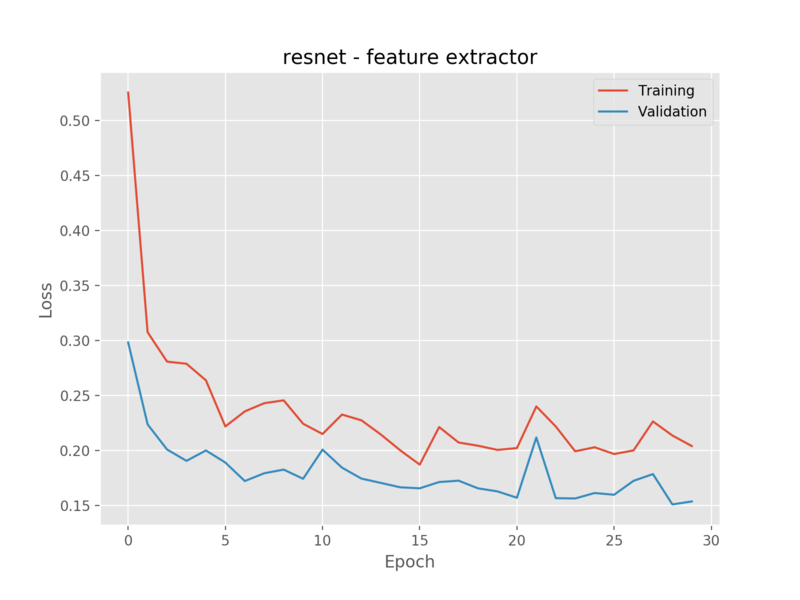
\includegraphics[width=9cm]{b_l_resnet_fe}
    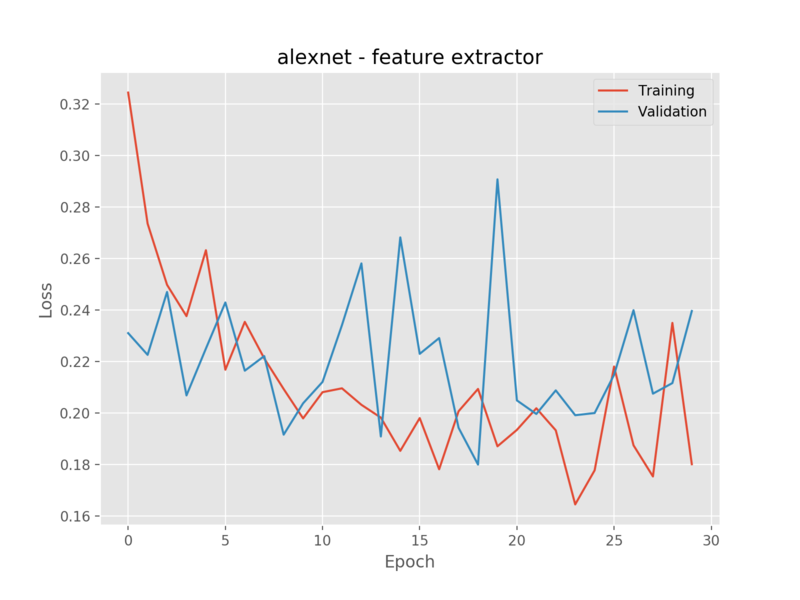
\includegraphics[width=9cm]{b_l_alexnet_fe}
    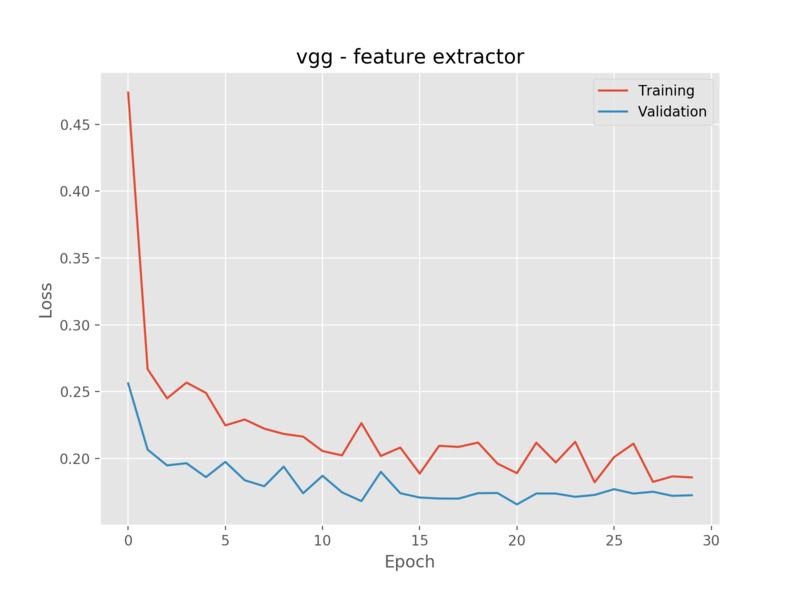
\includegraphics[width=9cm]{b_l_vgg_fe}
    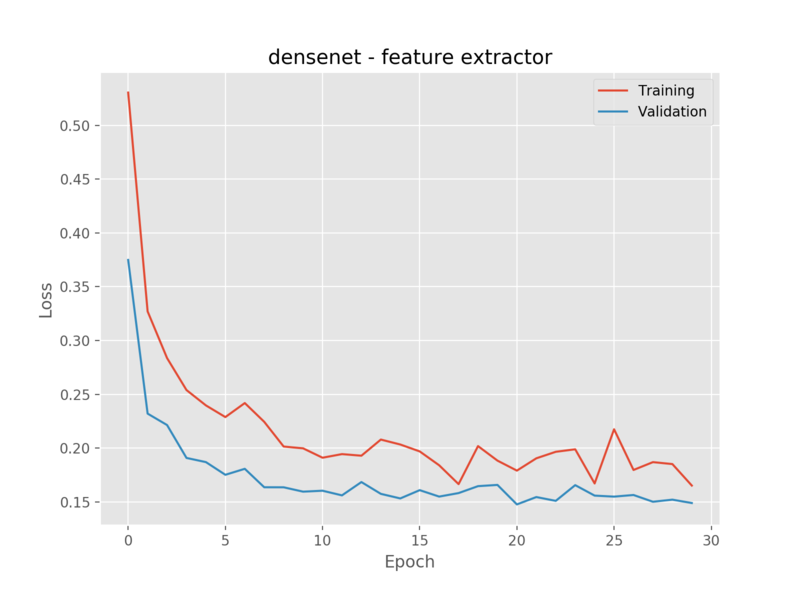
\includegraphics[width=9cm]{b_l_densenet_fe}
    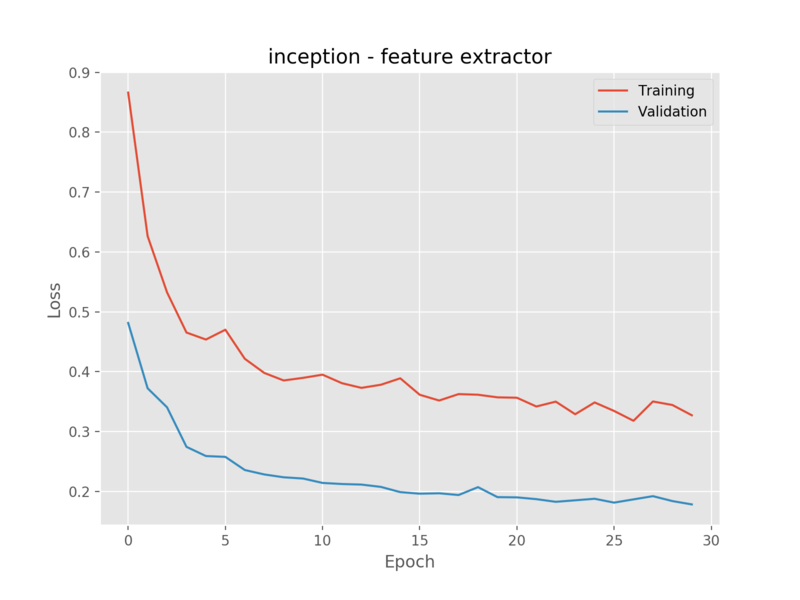
\includegraphics[width=9cm]{b_l_inception_fe}
    \caption{Kostnaden vid varje epoch för balkonger med feature extraction}
    \label{fig:b_l_1}
  \end{figure}
  
  \begin{figure}[h]
    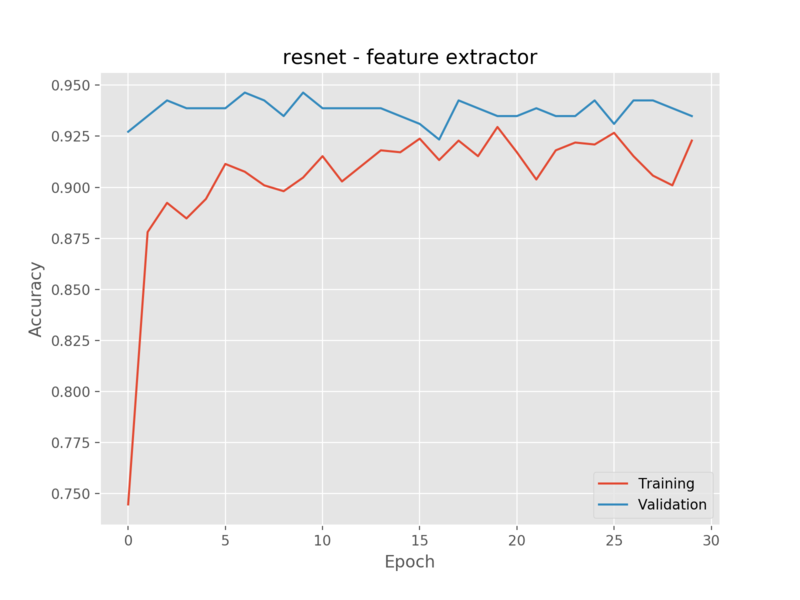
\includegraphics[width=9cm]{b_a_resnet_fe}
    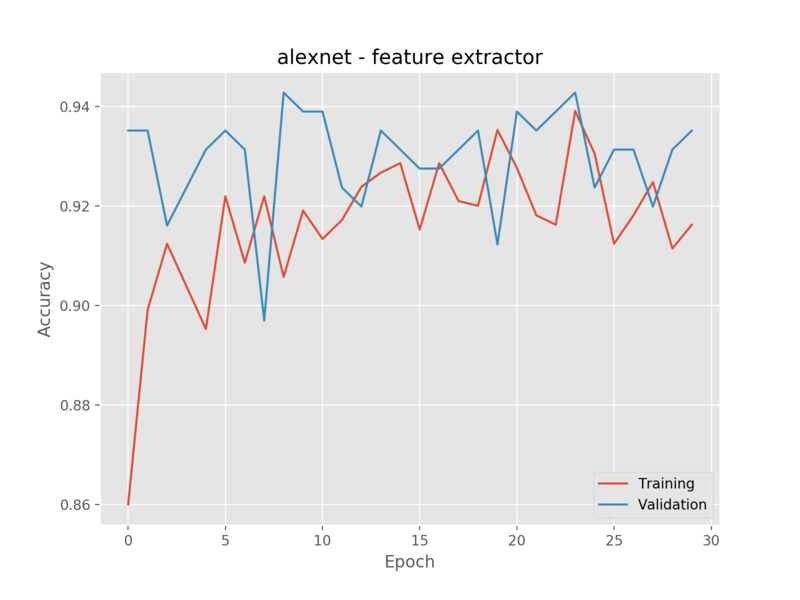
\includegraphics[width=9cm]{b_a_alexnet_fe}
    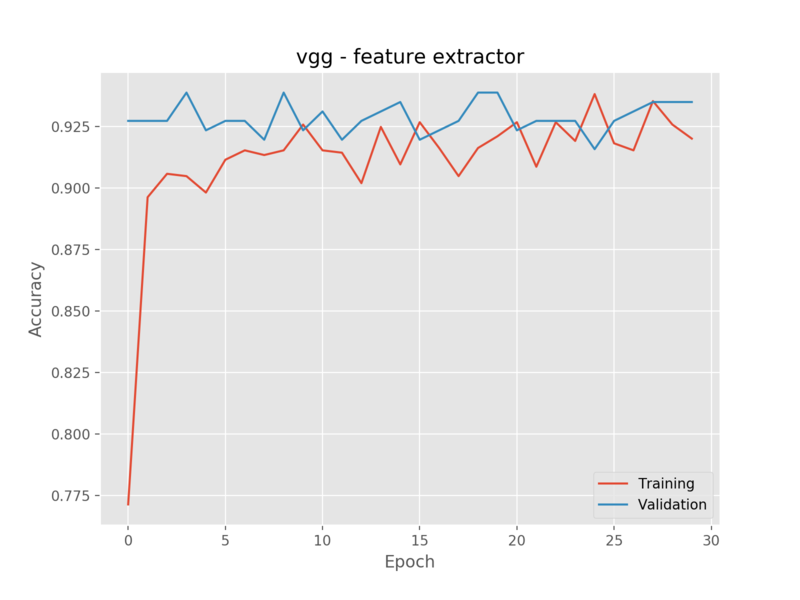
\includegraphics[width=9cm]{b_a_vgg_fe}
    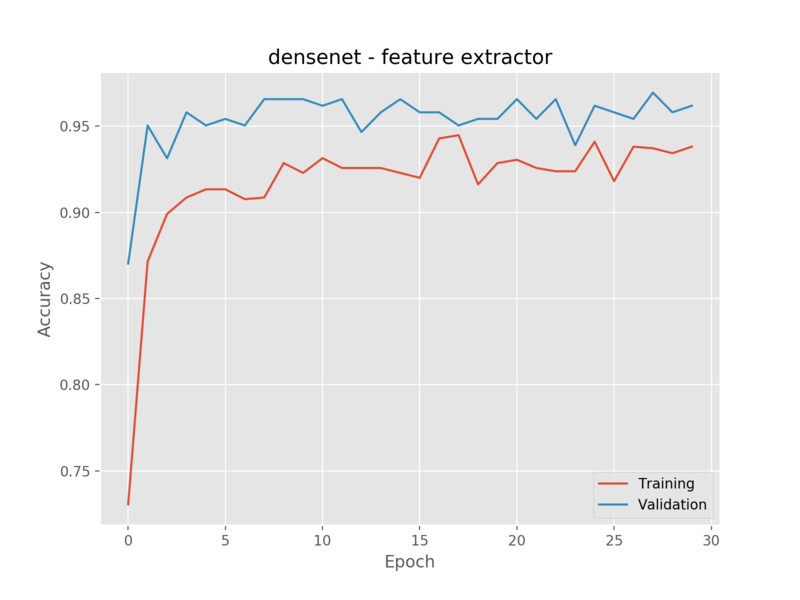
\includegraphics[width=9cm]{b_a_densenet_fe}
    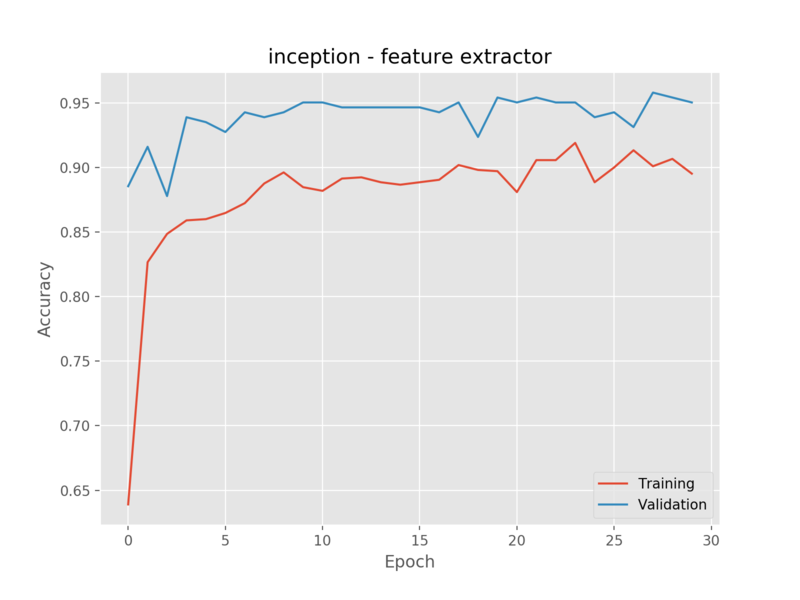
\includegraphics[width=9cm]{b_a_inception_fe}
    \caption{Träffsäkerhet för balkonger med feature extraction}
    \label{fig:b_a_1}
  \end{figure}
  
  \begin{figure}[h]
    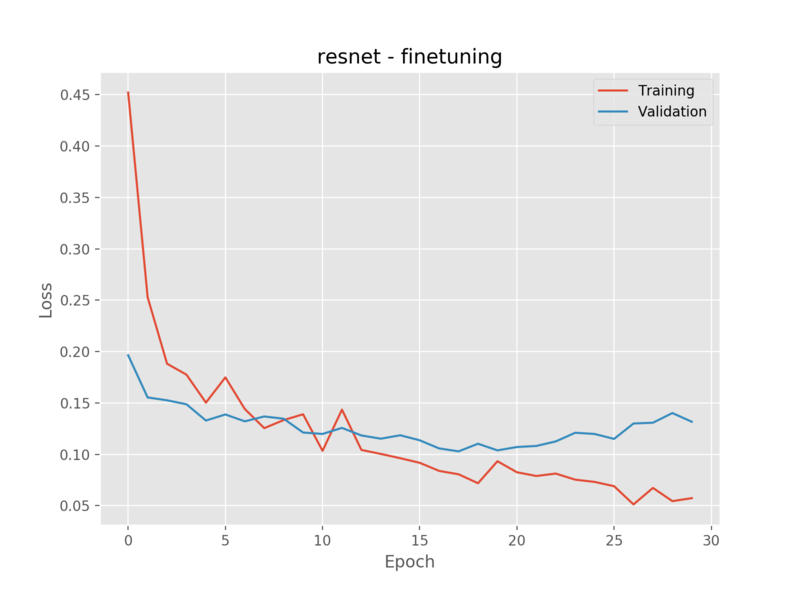
\includegraphics[width=9cm]{b_l_resnet_fine}
    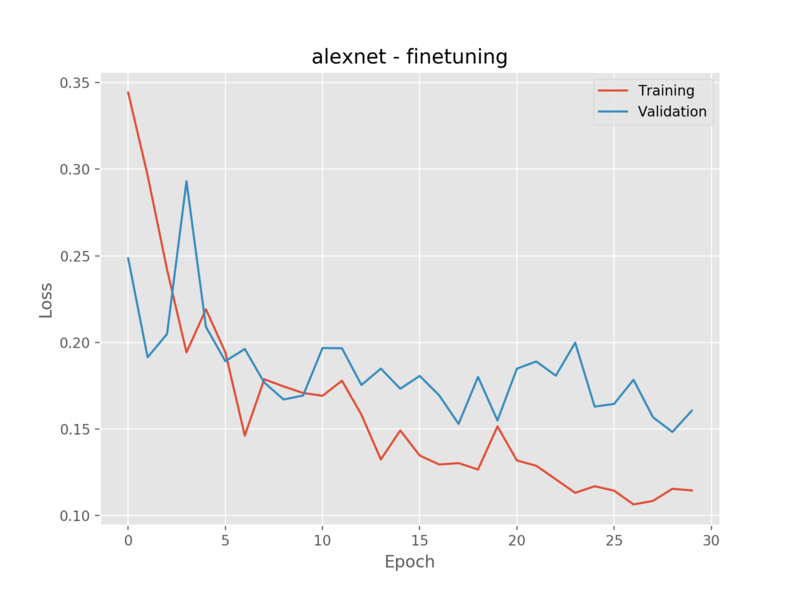
\includegraphics[width=9cm]{b_l_alexnet_fine}
    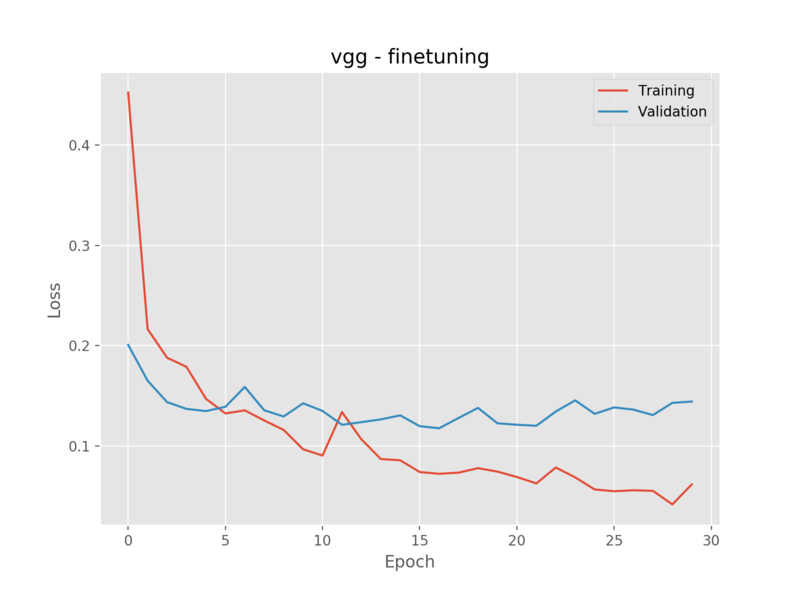
\includegraphics[width=9cm]{b_l_vgg_fine}
    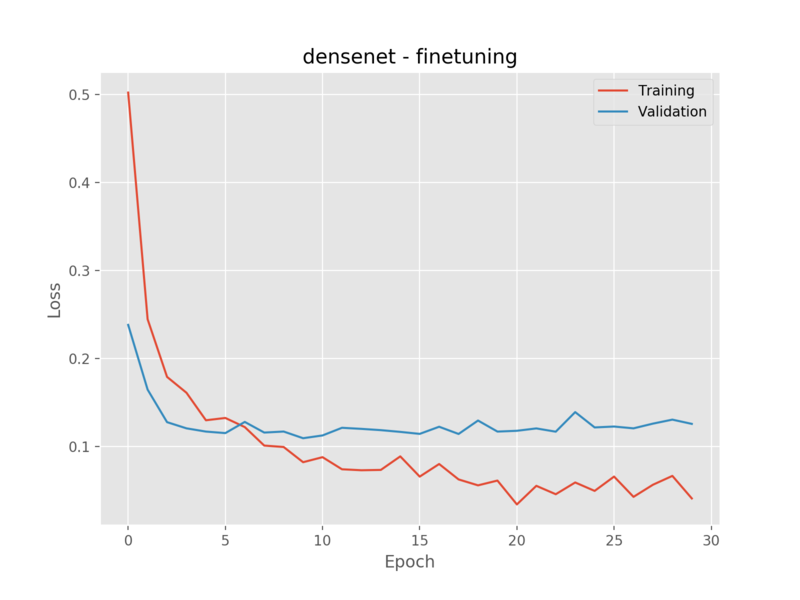
\includegraphics[width=9cm]{b_l_densenet_fine}
    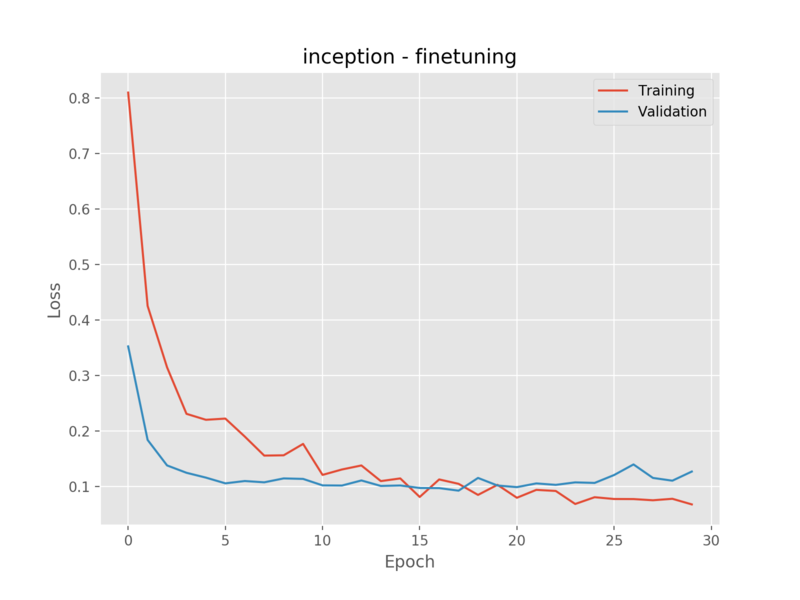
\includegraphics[width=9cm]{b_l_inception_fine}
    \caption{Kostnaden vid varje epoch för balkonger med finetuning}
    \label{fig:b_l_2}
  \end{figure}
  
  \begin{figure}[h]
    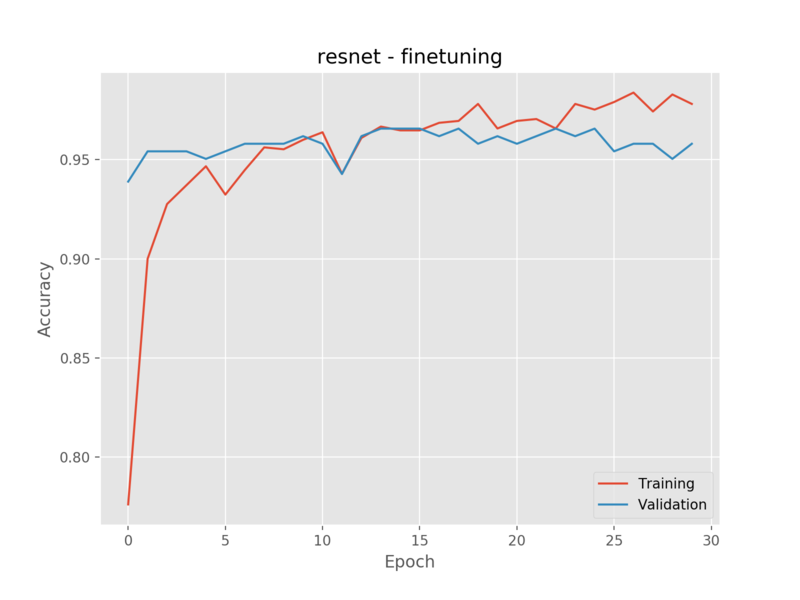
\includegraphics[width=9cm]{b_a_resnet_fine}
    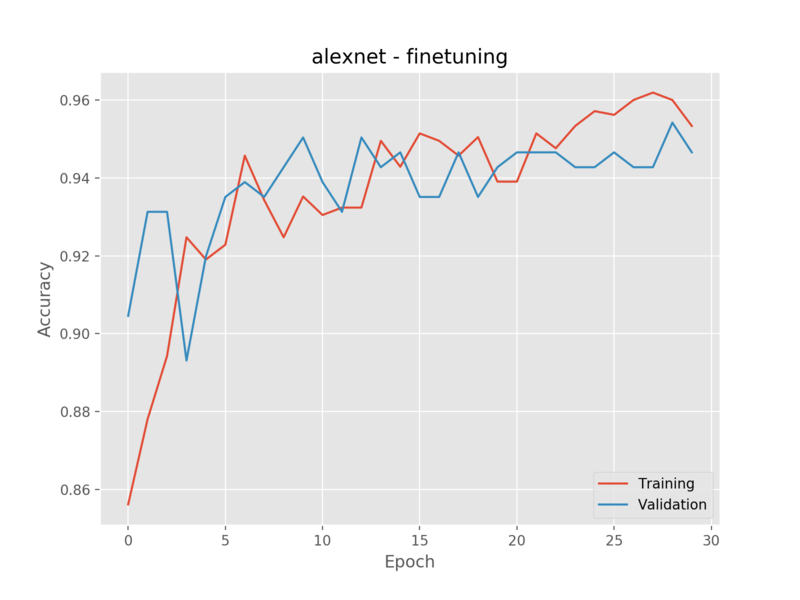
\includegraphics[width=9cm]{b_a_alexnet_fine}
    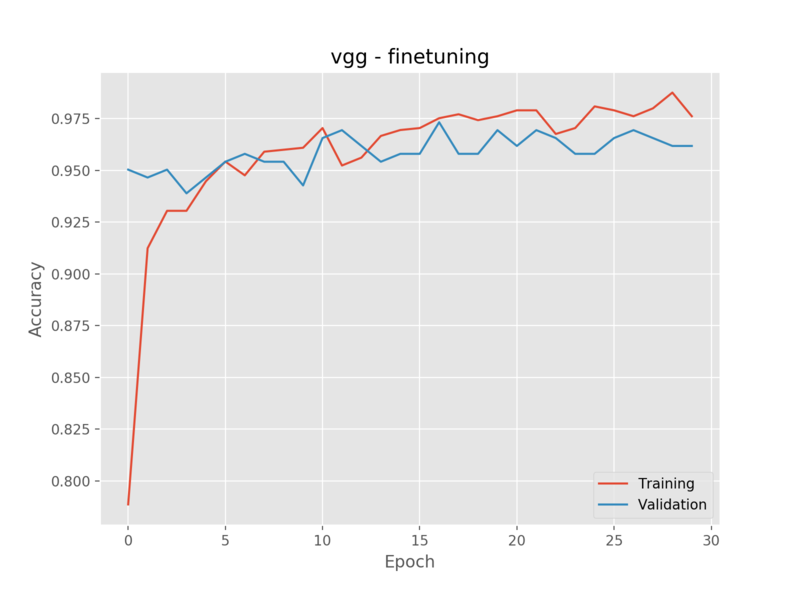
\includegraphics[width=9cm]{b_a_vgg_fine}
    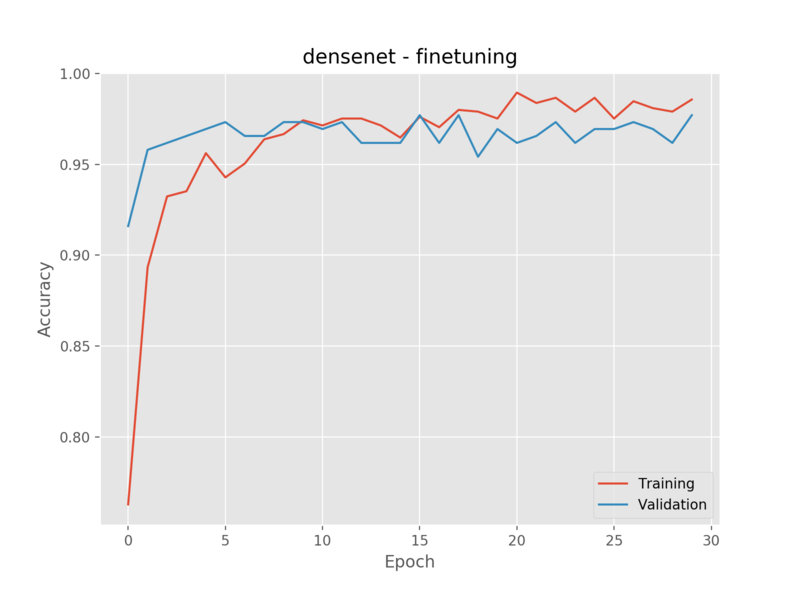
\includegraphics[width=9cm]{b_a_densenet_fine}
    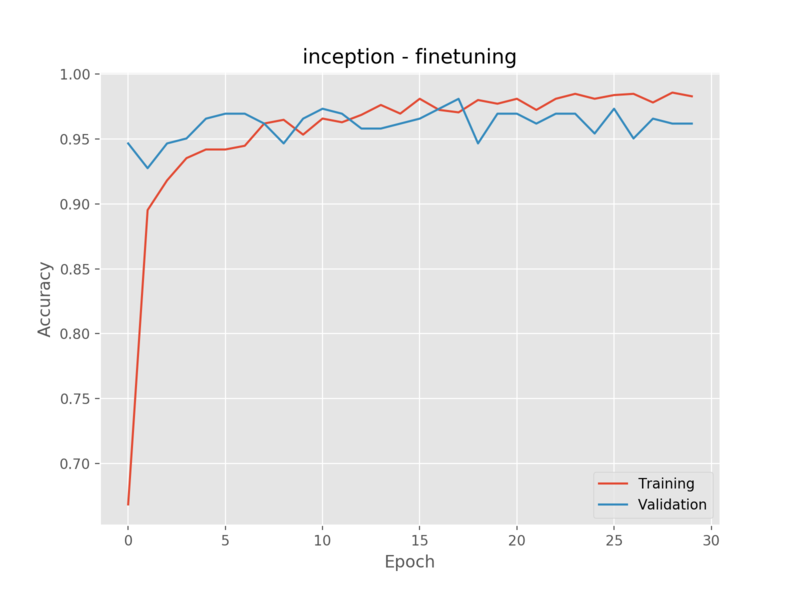
\includegraphics[width=9cm]{b_a_inception_fine}
    \caption{Träffsäkerhet för balkonger med finetuning}
    \label{fig:b_a_2}
  \end{figure}

  \begin{figure}[h]
    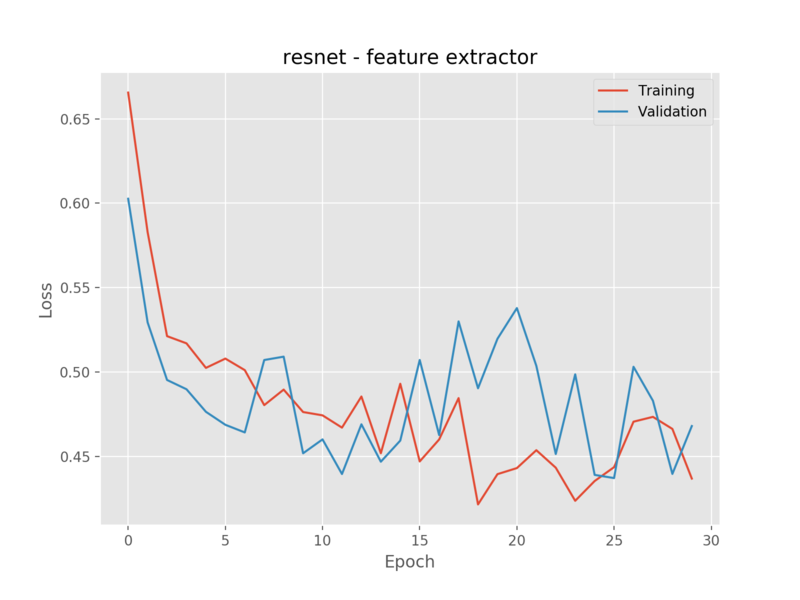
\includegraphics[width=9cm]{f_l_resnet_fe}
    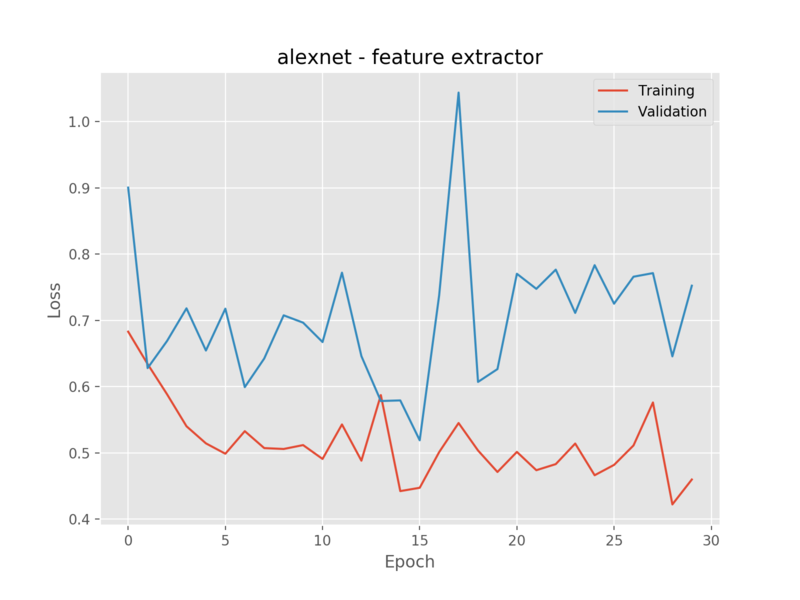
\includegraphics[width=9cm]{f_l_alexnet_fe}
    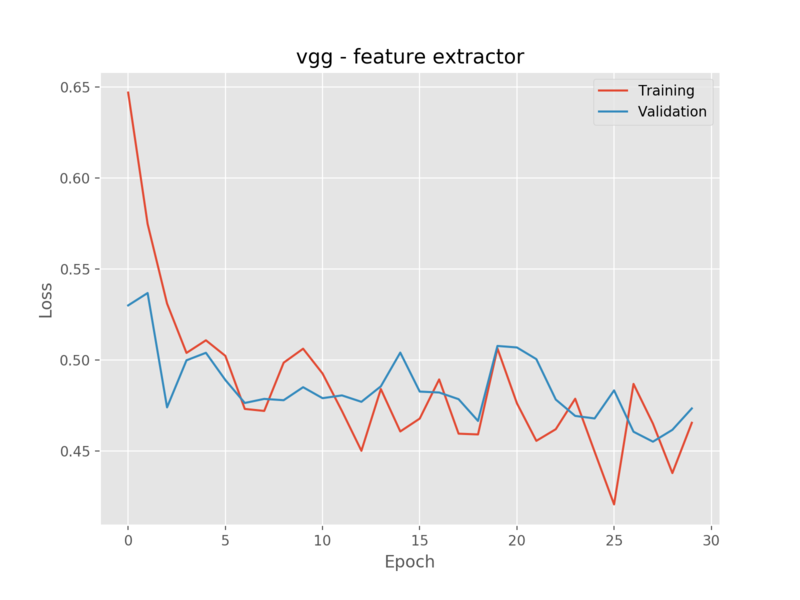
\includegraphics[width=9cm]{f_l_vgg_fe}
    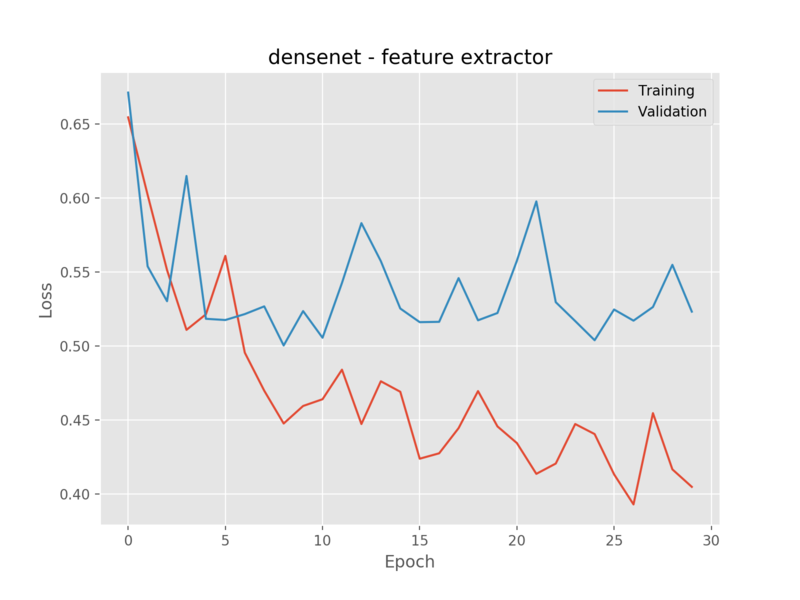
\includegraphics[width=9cm]{f_l_densenet_fe}
    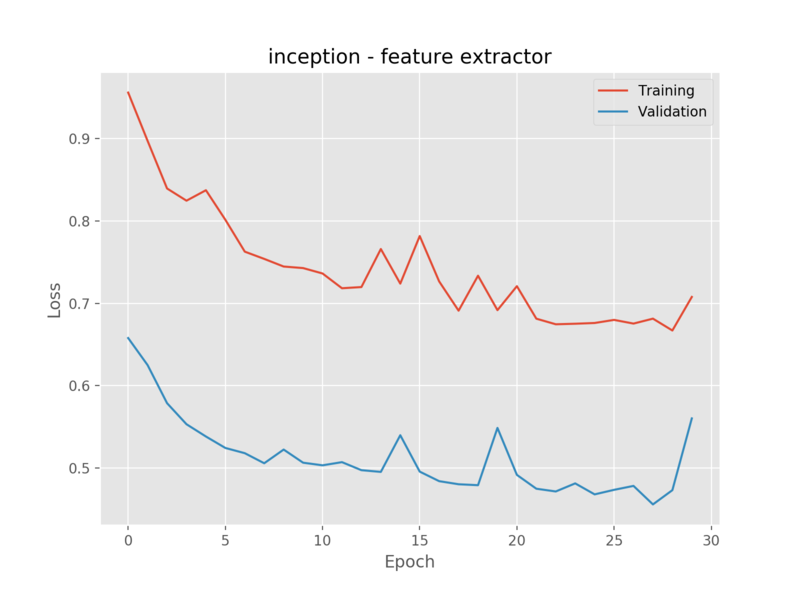
\includegraphics[width=9cm]{f_l_inception_fe}
    \caption{Kostnaden vid varje epoch för eldstäder med feature extraction}
    \label{fig:f_l_1}
  \end{figure}
  
  \begin{figure}[h]
    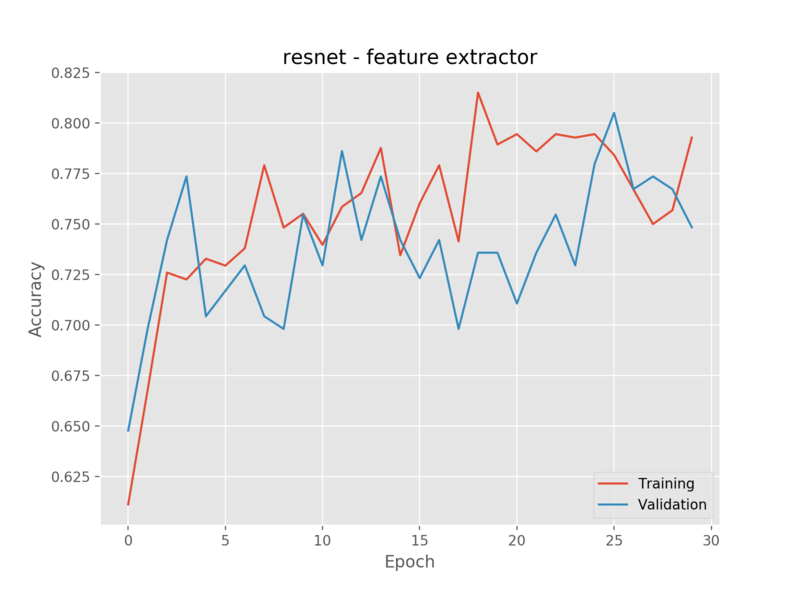
\includegraphics[width=9cm]{f_a_resnet_fe}
    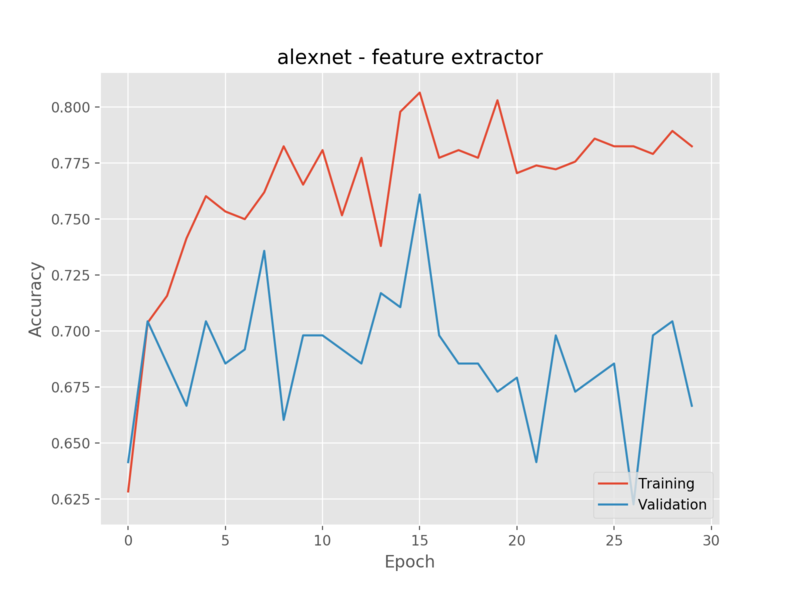
\includegraphics[width=9cm]{f_a_alexnet_fe}
    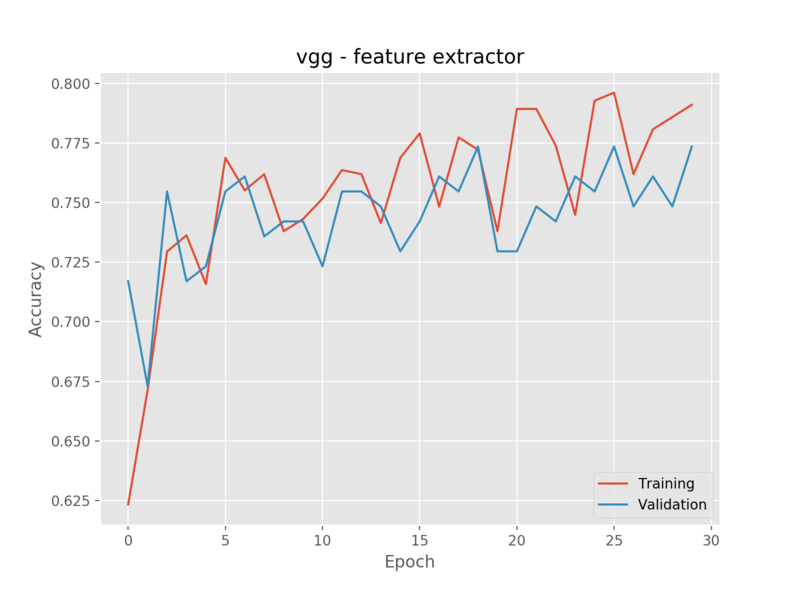
\includegraphics[width=9cm]{f_a_vgg_fe}
    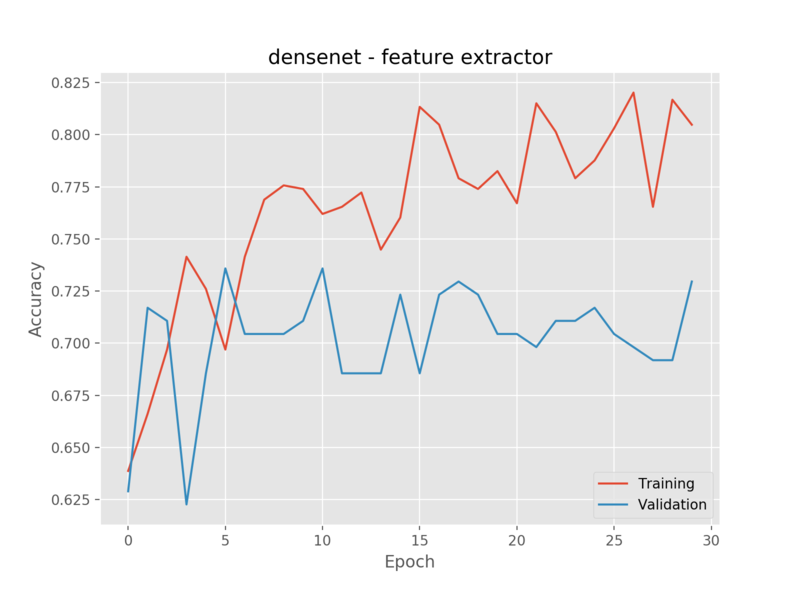
\includegraphics[width=9cm]{f_a_densenet_fe}
    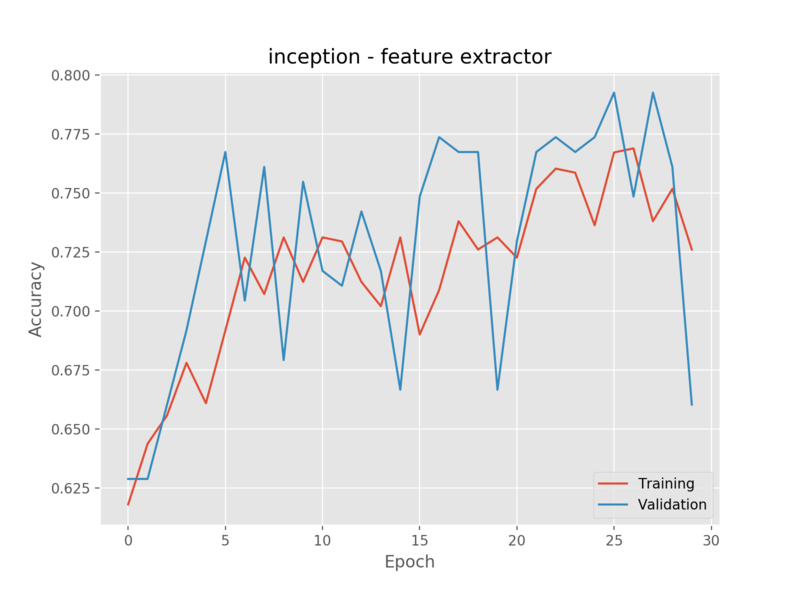
\includegraphics[width=9cm]{f_a_inception_fe}
    \caption{Träffsäkerhet för eldstäder med feature extraction}
    \label{fig:f_a_1}
  \end{figure}

  \begin{figure}[h]
    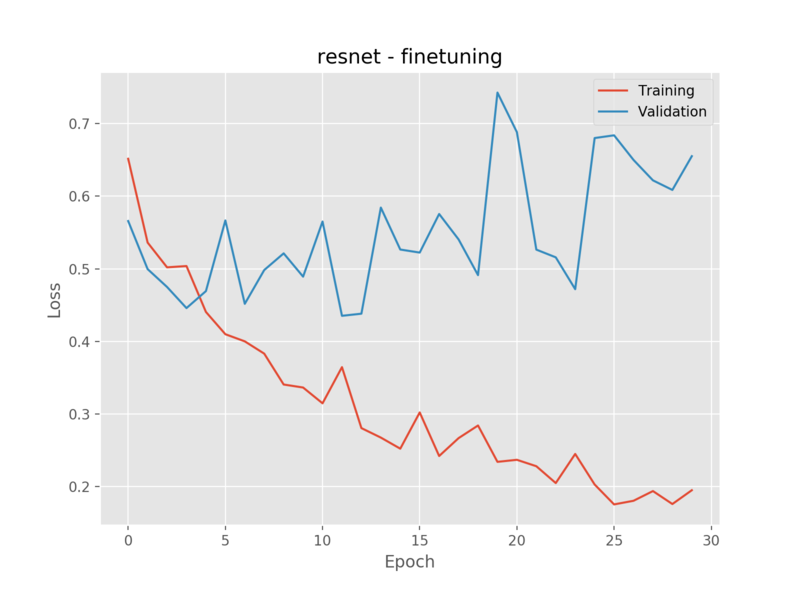
\includegraphics[width=9cm]{f_l_resnet_fine}
    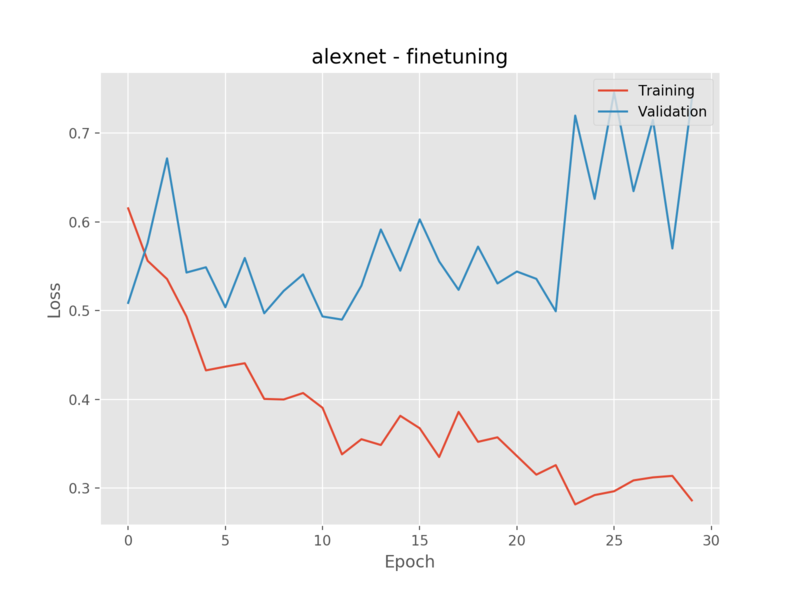
\includegraphics[width=9cm]{f_l_alexnet_fine}
    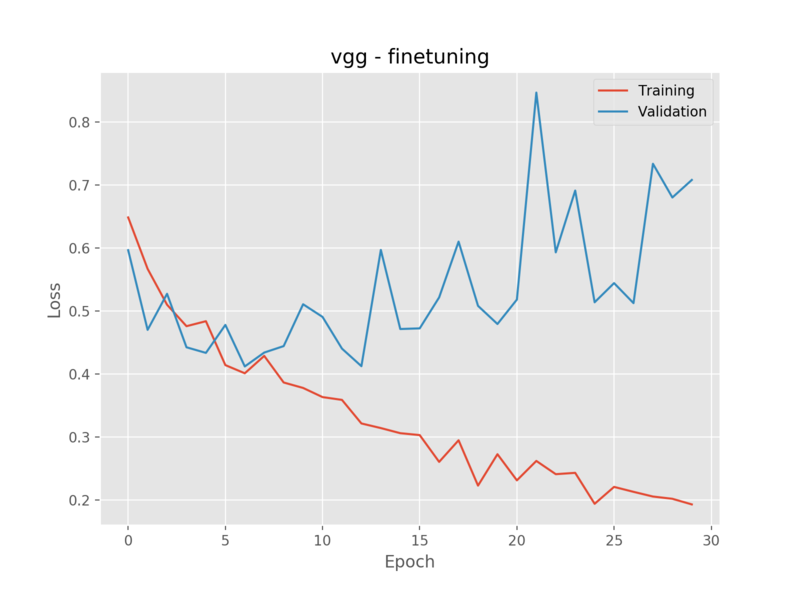
\includegraphics[width=9cm]{f_l_vgg_fine}
    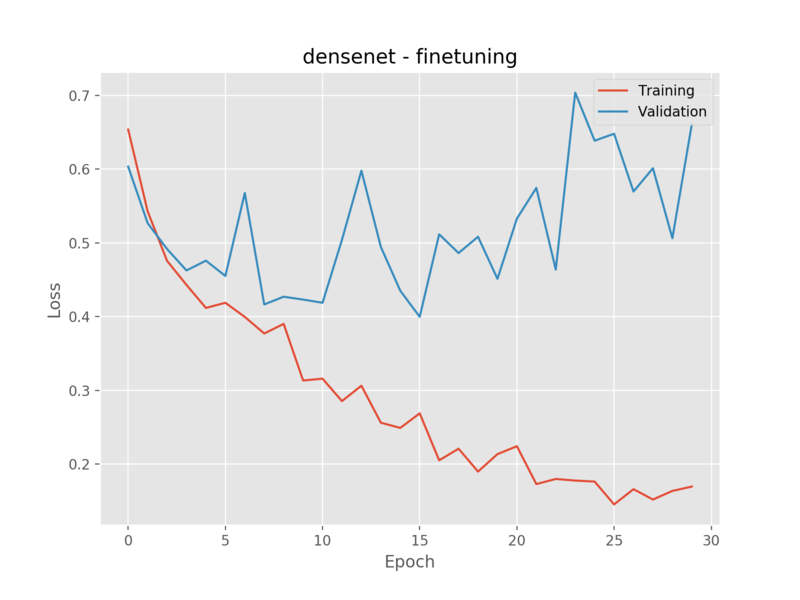
\includegraphics[width=9cm]{f_l_densenet_fine}
    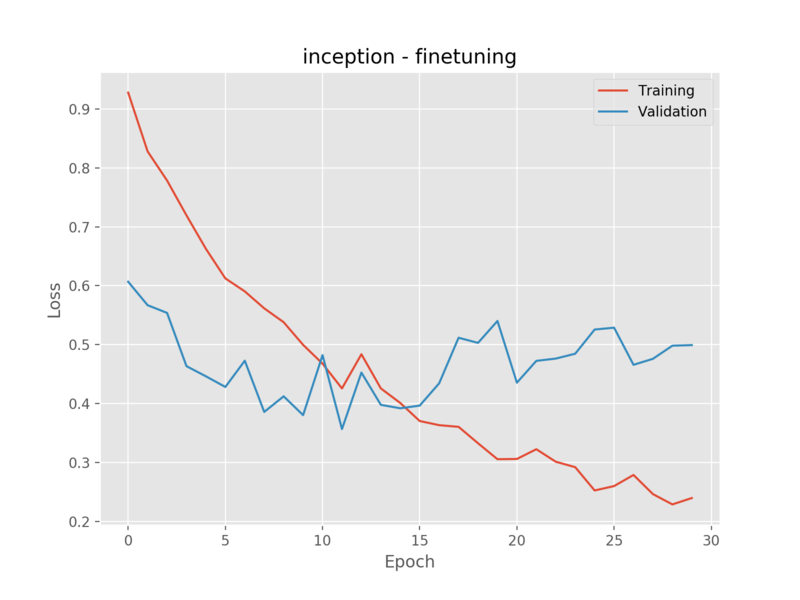
\includegraphics[width=9cm]{f_l_inception_fine}
    \caption{Kostnaden vid varje epoch för eldstäder med finetuning}
    \label{fig:f_l_2}
  \end{figure}

  \begin{figure}[h]
    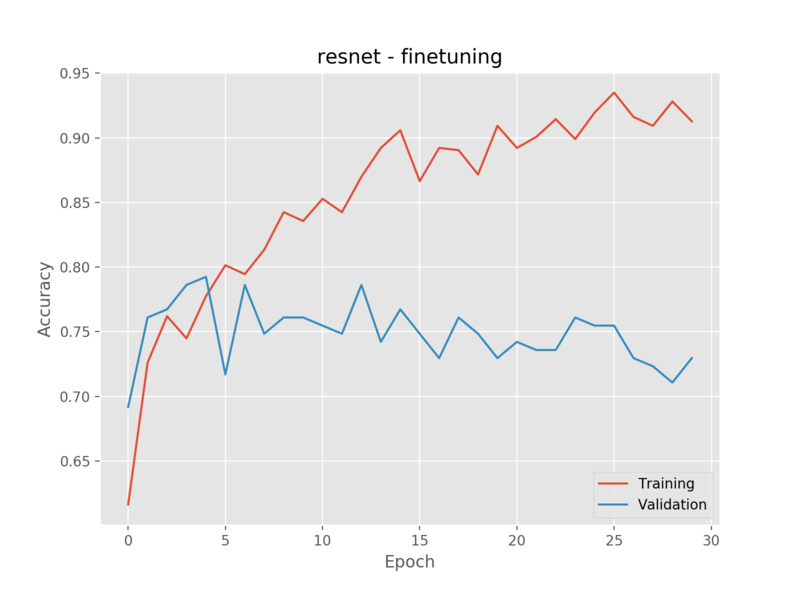
\includegraphics[width=9cm]{f_a_resnet_fine}
    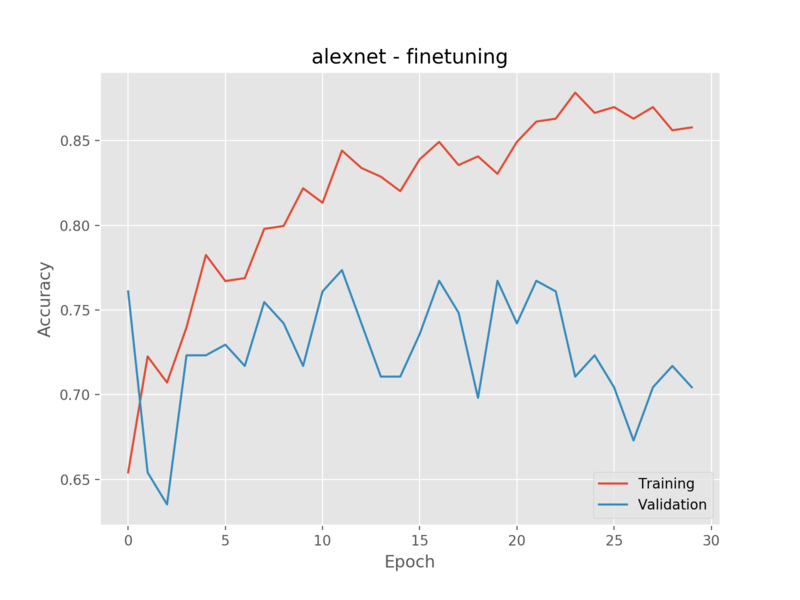
\includegraphics[width=9cm]{f_a_alexnet_fine}
    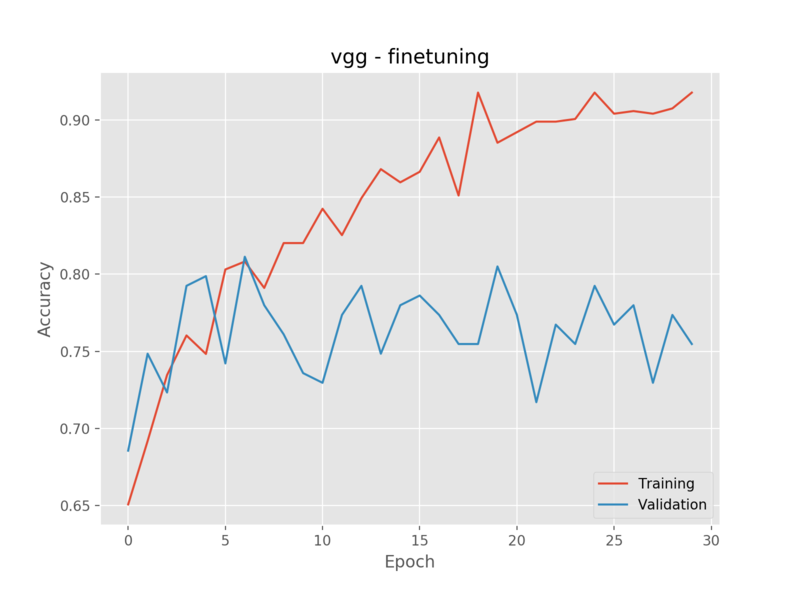
\includegraphics[width=9cm]{f_a_vgg_fine}
    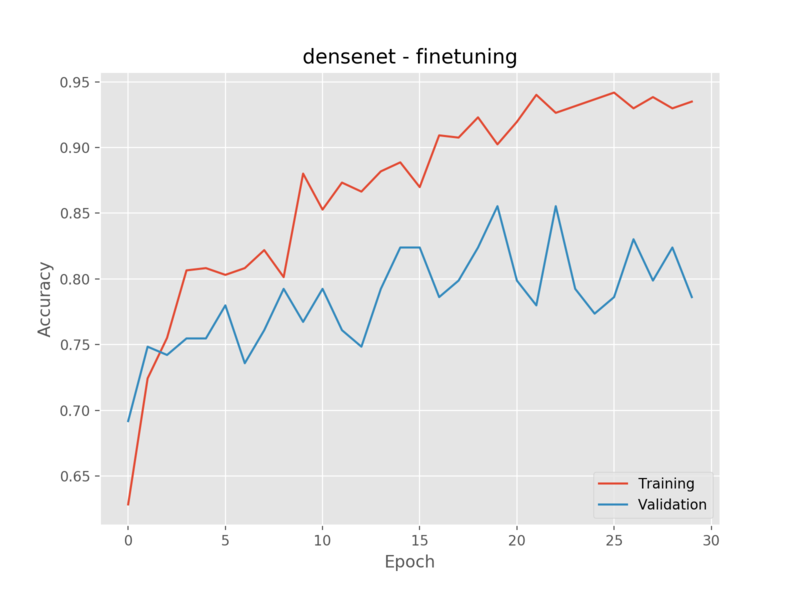
\includegraphics[width=9cm]{f_a_densenet_fine}
    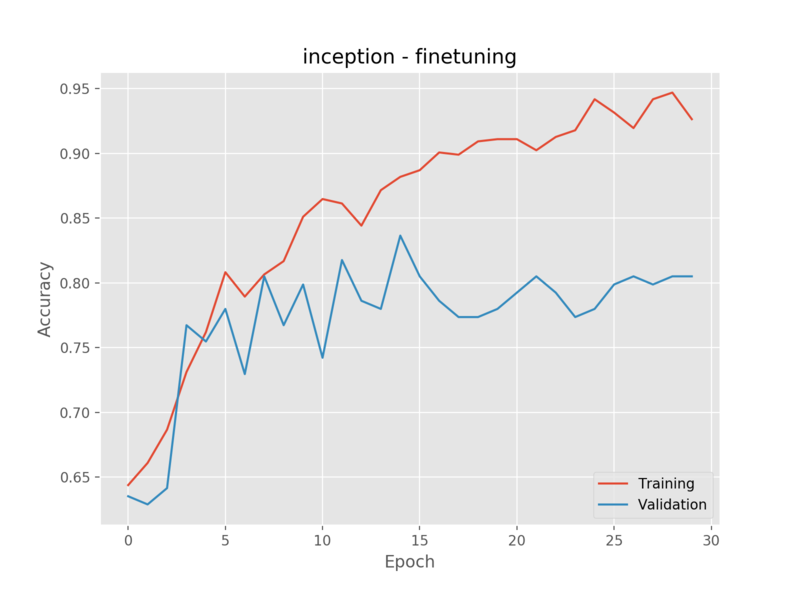
\includegraphics[width=9cm]{f_a_inception_fine}
    \caption{Träffsäkerhet för eldstäder med finetuning}
    \label{fig:f_a_2}
  \end{figure}
  
  \begin{figure}[h]
    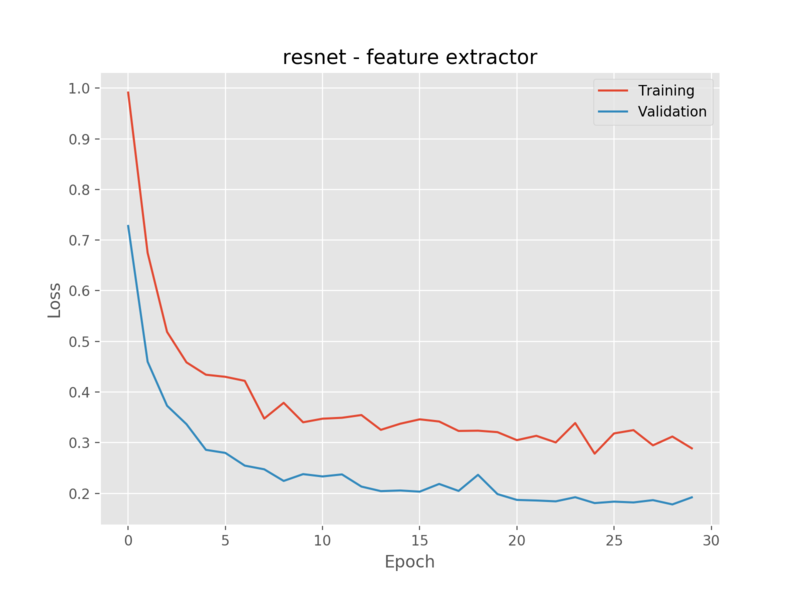
\includegraphics[width=9cm]{r_l_resnet_fe}
    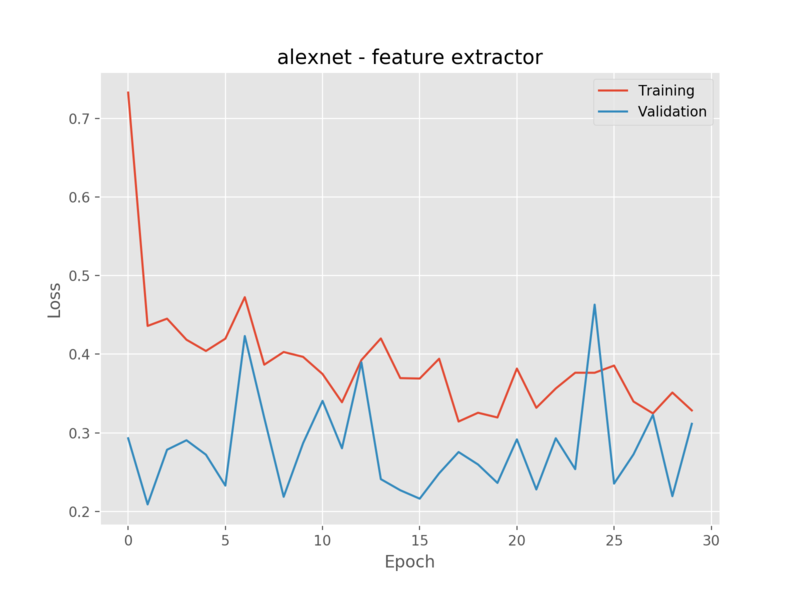
\includegraphics[width=9cm]{r_l_alexnet_fe}
    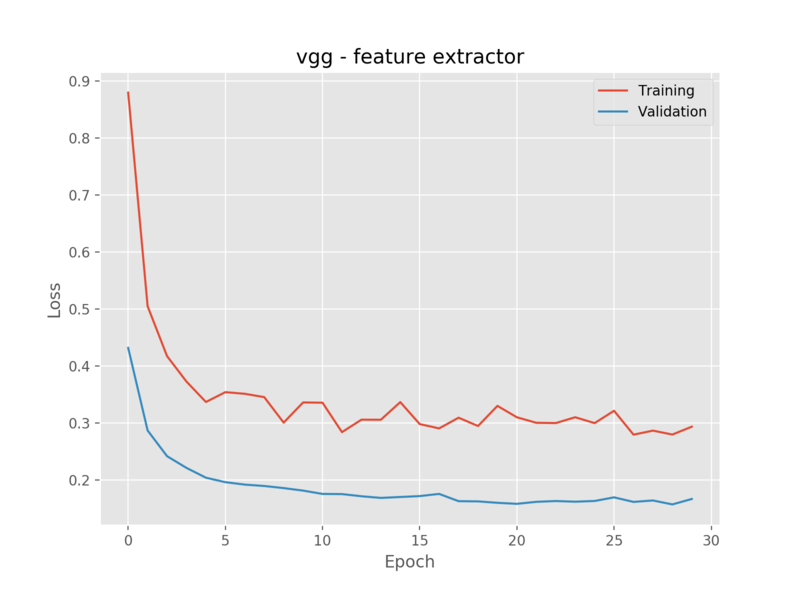
\includegraphics[width=9cm]{r_l_vgg_fe}
    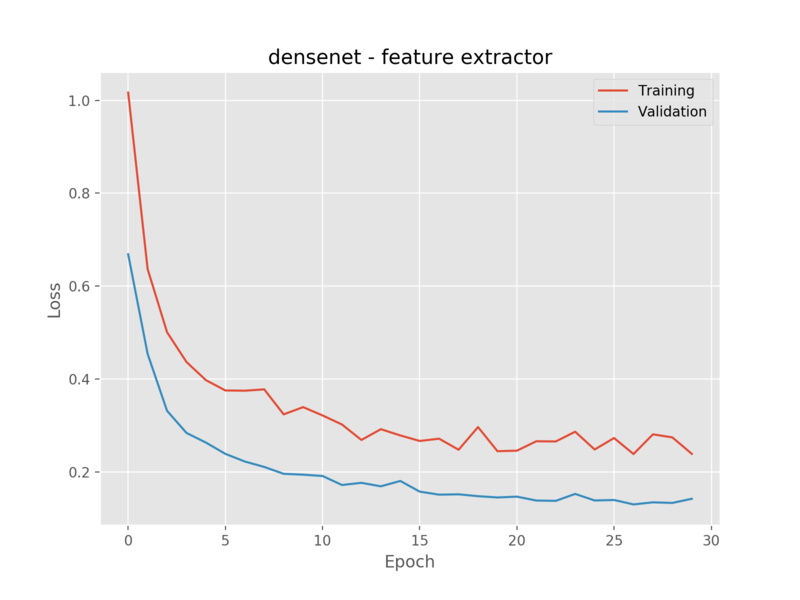
\includegraphics[width=9cm]{r_l_densenet_fe}
    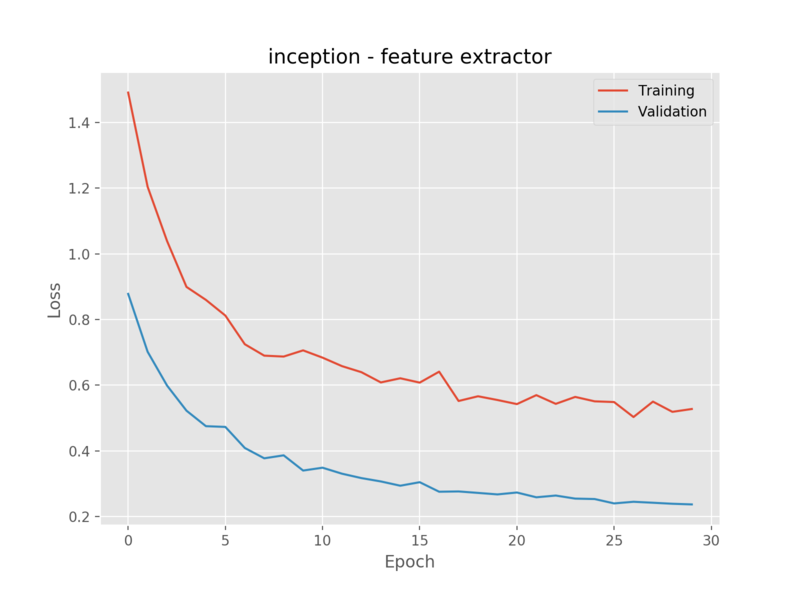
\includegraphics[width=9cm]{r_l_inception_fe}
    \caption{Kostnaden vid varje epoch för rum med feature extraction}
    \label{fig:r_l_1}
  \end{figure}
  
  \begin{figure}[h]
    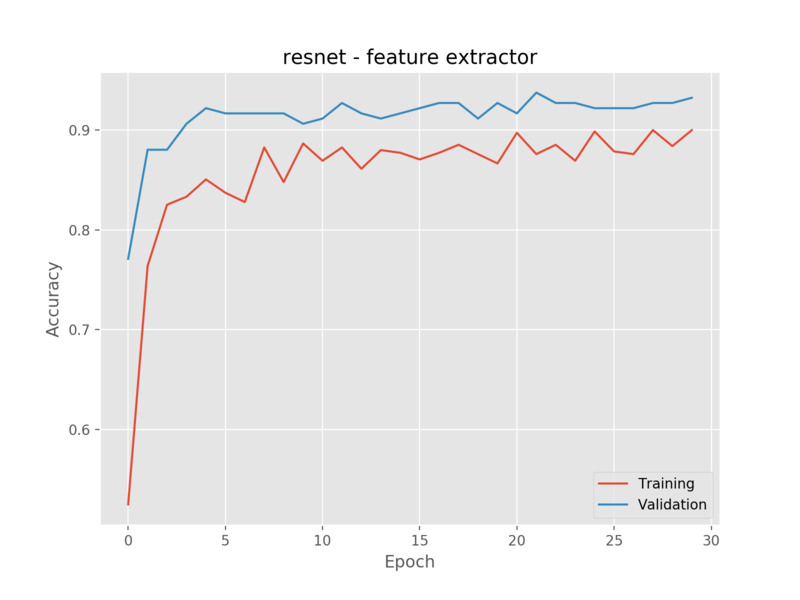
\includegraphics[width=9cm]{r_a_resnet_fe}
    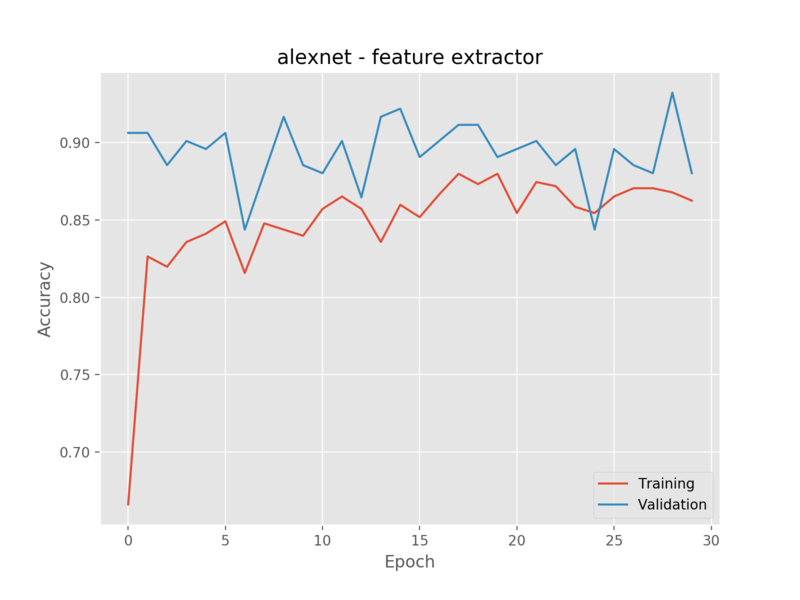
\includegraphics[width=9cm]{r_a_alexnet_fe}
    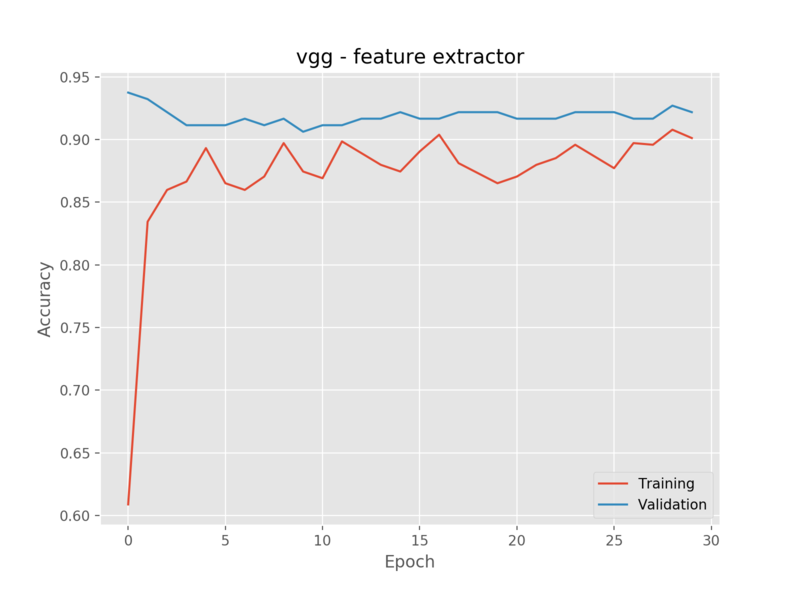
\includegraphics[width=9cm]{r_a_vgg_fe}
    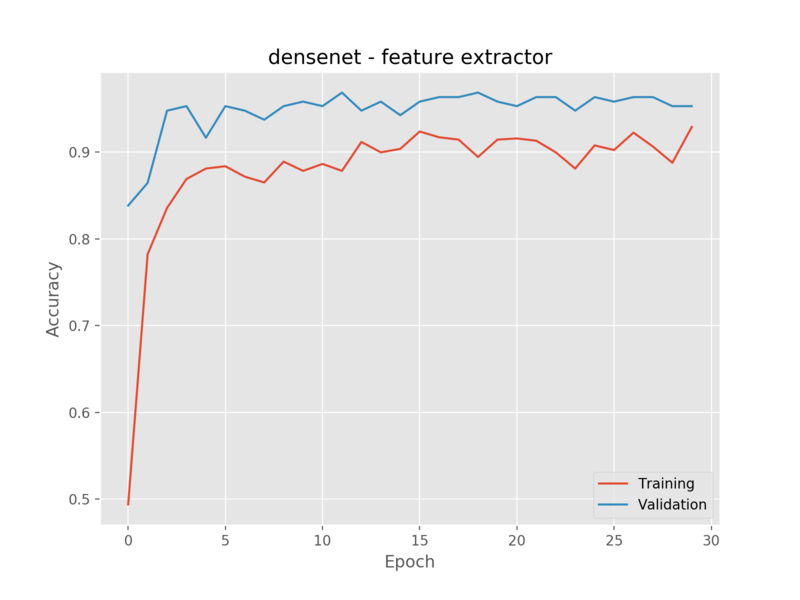
\includegraphics[width=9cm]{r_a_densenet_fe}
    \includegraphics[width=9cm]{r_a_inception_fe}
    \caption{Träffsäkerhet för rum med feature extraction}
    \label{fig:r_a_1}
  \end{figure}
  
  \begin{figure}[h]
    \includegraphics[width=9cm]{r_l_resnet_fine}
    \includegraphics[width=9cm]{r_l_alexnet_fine}
    \includegraphics[width=9cm]{r_l_vgg_fine}
    \includegraphics[width=9cm]{r_l_densenet_fine}
    \includegraphics[width=9cm]{r_l_inception_fine}
    \caption{Kostnaden vid varje epoch för rum med finetuning}
    \label{fig:r_l_2}
  \end{figure}
  
  \begin{figure}[h]
    \includegraphics[width=9cm]{r_a_resnet_fine}
    \includegraphics[width=9cm]{r_a_alexnet_fine}
    \includegraphics[width=9cm]{r_a_vgg_fine}
    \includegraphics[width=9cm]{r_a_densenet_fine}
    \includegraphics[width=9cm]{r_a_inception_fine}
    \caption{Träffsäkerhet för rum med finetuning}
    \label{fig:r_a_2}
  \end{figure}

\tailmatter
\end{document}
